% Options for packages loaded elsewhere
\PassOptionsToPackage{unicode}{hyperref}
\PassOptionsToPackage{hyphens}{url}
\PassOptionsToPackage{dvipsnames,svgnames,x11names}{xcolor}
%
\documentclass[
  letterpaper,
]{scrbook}

\usepackage{amsmath,amssymb}
\usepackage{iftex}
\ifPDFTeX
  \usepackage[T1]{fontenc}
  \usepackage[utf8]{inputenc}
  \usepackage{textcomp} % provide euro and other symbols
\else % if luatex or xetex
  \usepackage{unicode-math}
  \defaultfontfeatures{Scale=MatchLowercase}
  \defaultfontfeatures[\rmfamily]{Ligatures=TeX,Scale=1}
\fi
\usepackage{lmodern}
\ifPDFTeX\else  
    % xetex/luatex font selection
  \setmainfont[]{TeX Gyre Termes}
  \setsansfont[]{TeX Gyre Heros}
  \setmonofont[]{TeX Gyre Cursor}
  \setmathfont[]{TeX Gyre Termes}
\fi
% Use upquote if available, for straight quotes in verbatim environments
\IfFileExists{upquote.sty}{\usepackage{upquote}}{}
\IfFileExists{microtype.sty}{% use microtype if available
  \usepackage[]{microtype}
  \UseMicrotypeSet[protrusion]{basicmath} % disable protrusion for tt fonts
}{}
\makeatletter
\@ifundefined{KOMAClassName}{% if non-KOMA class
  \IfFileExists{parskip.sty}{%
    \usepackage{parskip}
  }{% else
    \setlength{\parindent}{0pt}
    \setlength{\parskip}{6pt plus 2pt minus 1pt}}
}{% if KOMA class
  \KOMAoptions{parskip=half}}
\makeatother
\usepackage{xcolor}
\usepackage[left=1in,marginparwidth=2.0666666666667in,textwidth=4.1333333333333in,marginparsep=0.3in]{geometry}
\setlength{\emergencystretch}{3em} % prevent overfull lines
\setcounter{secnumdepth}{5}
% Make \paragraph and \subparagraph free-standing
\ifx\paragraph\undefined\else
  \let\oldparagraph\paragraph
  \renewcommand{\paragraph}[1]{\oldparagraph{#1}\mbox{}}
\fi
\ifx\subparagraph\undefined\else
  \let\oldsubparagraph\subparagraph
  \renewcommand{\subparagraph}[1]{\oldsubparagraph{#1}\mbox{}}
\fi


\providecommand{\tightlist}{%
  \setlength{\itemsep}{0pt}\setlength{\parskip}{0pt}}\usepackage{longtable,booktabs,array}
\usepackage{calc} % for calculating minipage widths
% Correct order of tables after \paragraph or \subparagraph
\usepackage{etoolbox}
\makeatletter
\patchcmd\longtable{\par}{\if@noskipsec\mbox{}\fi\par}{}{}
\makeatother
% Allow footnotes in longtable head/foot
\IfFileExists{footnotehyper.sty}{\usepackage{footnotehyper}}{\usepackage{footnote}}
\makesavenoteenv{longtable}
\usepackage{graphicx}
\makeatletter
\def\maxwidth{\ifdim\Gin@nat@width>\linewidth\linewidth\else\Gin@nat@width\fi}
\def\maxheight{\ifdim\Gin@nat@height>\textheight\textheight\else\Gin@nat@height\fi}
\makeatother
% Scale images if necessary, so that they will not overflow the page
% margins by default, and it is still possible to overwrite the defaults
% using explicit options in \includegraphics[width, height, ...]{}
\setkeys{Gin}{width=\maxwidth,height=\maxheight,keepaspectratio}
% Set default figure placement to htbp
\makeatletter
\def\fps@figure{htbp}
\makeatother
% definitions for citeproc citations
\NewDocumentCommand\citeproctext{}{}
\NewDocumentCommand\citeproc{mm}{%
  \begingroup\def\citeproctext{#2}\cite{#1}\endgroup}
\makeatletter
 % allow citations to break across lines
 \let\@cite@ofmt\@firstofone
 % avoid brackets around text for \cite:
 \def\@biblabel#1{}
 \def\@cite#1#2{{#1\if@tempswa , #2\fi}}
\makeatother
\newlength{\cslhangindent}
\setlength{\cslhangindent}{1.5em}
\newlength{\csllabelwidth}
\setlength{\csllabelwidth}{3em}
\newenvironment{CSLReferences}[2] % #1 hanging-indent, #2 entry-spacing
 {\begin{list}{}{%
  \setlength{\itemindent}{0pt}
  \setlength{\leftmargin}{0pt}
  \setlength{\parsep}{0pt}
  % turn on hanging indent if param 1 is 1
  \ifodd #1
   \setlength{\leftmargin}{\cslhangindent}
   \setlength{\itemindent}{-1\cslhangindent}
  \fi
  % set entry spacing
  \setlength{\itemsep}{#2\baselineskip}}}
 {\end{list}}
\usepackage{calc}
\newcommand{\CSLBlock}[1]{\hfill\break#1\hfill\break}
\newcommand{\CSLLeftMargin}[1]{\parbox[t]{\csllabelwidth}{\strut#1\strut}}
\newcommand{\CSLRightInline}[1]{\parbox[t]{\linewidth - \csllabelwidth}{\strut#1\strut}}
\newcommand{\CSLIndent}[1]{\hspace{\cslhangindent}#1}

\makeatletter
\@ifpackageloaded{bookmark}{}{\usepackage{bookmark}}
\makeatother
\makeatletter
\@ifpackageloaded{caption}{}{\usepackage{caption}}
\AtBeginDocument{%
\ifdefined\contentsname
  \renewcommand*\contentsname{Table of contents}
\else
  \newcommand\contentsname{Table of contents}
\fi
\ifdefined\listfigurename
  \renewcommand*\listfigurename{List of Figures}
\else
  \newcommand\listfigurename{List of Figures}
\fi
\ifdefined\listtablename
  \renewcommand*\listtablename{List of Tables}
\else
  \newcommand\listtablename{List of Tables}
\fi
\ifdefined\figurename
  \renewcommand*\figurename{Figure}
\else
  \newcommand\figurename{Figure}
\fi
\ifdefined\tablename
  \renewcommand*\tablename{Table}
\else
  \newcommand\tablename{Table}
\fi
}
\@ifpackageloaded{float}{}{\usepackage{float}}
\floatstyle{ruled}
\@ifundefined{c@chapter}{\newfloat{codelisting}{h}{lop}}{\newfloat{codelisting}{h}{lop}[chapter]}
\floatname{codelisting}{Listing}
\newcommand*\listoflistings{\listof{codelisting}{List of Listings}}
\makeatother
\makeatletter
\@ifpackageloaded{caption}{}{\usepackage{caption}}
\@ifpackageloaded{subcaption}{}{\usepackage{subcaption}}
\makeatother
\makeatletter
\@ifpackageloaded{sidenotes}{}{\usepackage{sidenotes}}
\@ifpackageloaded{marginnote}{}{\usepackage{marginnote}}
\makeatother
\makeatletter
\makeatother
\ifLuaTeX
  \usepackage{selnolig}  % disable illegal ligatures
\fi
\IfFileExists{bookmark.sty}{\usepackage{bookmark}}{\usepackage{hyperref}}
\IfFileExists{xurl.sty}{\usepackage{xurl}}{} % add URL line breaks if available
\urlstyle{same} % disable monospaced font for URLs
\hypersetup{
  pdftitle={Data Science for Biodiversity Scientists},
  pdfauthor={Timothée Poisot},
  colorlinks=true,
  linkcolor={SteelBlue4},
  filecolor={Maroon},
  citecolor={Blue},
  urlcolor={Blue},
  pdfcreator={LaTeX via pandoc}}

\title{Data Science for Biodiversity Scientists}
\usepackage{etoolbox}
\makeatletter
\providecommand{\subtitle}[1]{% add subtitle to \maketitle
  \apptocmd{\@title}{\par {\large #1 \par}}{}{}
}
\makeatother
\subtitle{An introduction to concepts and practices}
\author{Timothée Poisot}
\date{2023-09-28}

\begin{document}
\frontmatter
\maketitle
\renewcommand*\contentsname{Table of contents}
{
\hypersetup{linkcolor=}
\setcounter{tocdepth}{1}
\tableofcontents
}
\mainmatter
\bookmarksetup{startatroot}

\chapter*{Preface}\label{preface}
\addcontentsline{toc}{chapter}{Preface}

\markboth{Preface}{Preface}

Data science is now an established methodology to study biodiversity,
and this is a problem.

This may be an opportunity when it comes to advancing our knowledge of
biodiversity, and in particular when it comes to translating this
knowledge into action (Tuia \emph{et al.} 2022); but make no mistake,
this is a problem for us, biodiversity scientists, as we suddenly need
to develop competences in an entirely new field. And as luck would have
it, there are easier fields to master than data science. The point of
this book, therefore, is to provide an introduction to fundamental
concepts in data science, from the perspective of a biodiversity
scientist, by using examples corresponding to real-world use-cases of
these techniques.

But what do we mean by \emph{data science}? Most science, after all,
relies on data in some capacity. What falls under the umbrella of data
science is, in short, embracing in equal measure quantitative skills
(mathematics, machine learning, statistics), programming, and domain
expertise, in order to solve well-defined problems. A core tenet of data
science is that, when using it, we seek to ``deliver actionable
insights'', which is MBA-speak for ``figuring out what to do next''. One
of the ways in which this occurs is by letting the data speak, after
they have been, of course, properly cleaned and transformed and
engineered beyond recognition. This entire process is driven by (or
subject to, even) domain knowledge. There is no such thing as data
science, at least not in a vacuum: there is data science as a
methodology applied to a specific domain.

Before we embark into a journey of discovery on the applications of data
science to biodiversity, allow me to let you in on a little secret: data
\emph{science} is a little bit of a misnomer.

To understand why, it helps to think of science (the application of the
scientific method, that is) as cooking. There are general techniques one
must master, and specific steps and cultural specifics, and there is a
final product. When writing this preface, I turned to my shelf of
cookbooks, and picked my two favorites: Robuchon's \emph{The Complete
Robuchon} (a no-nonsense list of hundreds of recipes with no place for
improvisation), and Bianco's \emph{Pizza, Pasta, and Other Food I Like}
(a short volume with very few pizza and pasta, and wonderful discussions
about the importance of humility, creativity, and generosity). Data
science, if it were cooking, would feel a lot like the second. Deviation
from the rules (they are mostly recommendations, in fact) is often
justifiable if you feel like it. But this improvisation requires good
skills, a clear mental map of the problem, and a library of patterns
that you can draw from.

This book will not get you here. But it will speed up the process, by
framing the practice of data science as a natural way to conduct
research on biodiversity.

\bookmarksetup{startatroot}

\chapter{Introduction}\label{introduction}

This book started as a collection of notes from several classes I gave
in the Department of Biological Sciences at the Université de Montréal,
as well as a few workshops I ran for the Québec Centre for Biodiversity
Sciences. In teaching data synthesis, data science, and machine learning
to biology students, I realized that the field was missing a stepping
stone to proficiency. There are excellent manuals covering the
mathematics of data science and machine learning; there are many good
papers giving overviews of some applications of data science to
biological problems; and there are, of course, thousands of tutorials
about how to write code (some of them are good!).

But one thing that students commonly called for was an attempt to tie
concepts together, and to explain when and how human decisions were
required in ML approaches (Sulmont \emph{et al.} 2019). This is this
attempt.

There are, broadly speaking, two situations in which reading this book
is useful. The first is when you are done reading some general books
about machine learning, and want to see how it can be applied to
problems that are more specific to biodiversity research; the second is
when you have a working understanding of biodiversity research, and want
a stepping stone into the machine learning literature. Note that there
is no scenario where you \emph{stop} after reading this book -- this is
by design. The purpose of this book is to give a practical overview of
``how data science for biodiversity happens'', and this needs to be done
in parallel to even more fundamental readings.

These are examples of books I like. I found them comprehensive and
engaging. They may not work for you.

A wonderful introduction to the mathematics behind machine learning can
be found in Deisenroth \emph{et al.} (2020), which provides stunning
visualization of mathematical concepts. Yau (2015) is a particularly
useful book about the ways to visualize data in a meaningful way.
\textbf{TK}

When reading this book, I encourage you to read the chapters in order.
They have been designed to be read in order, because each chapter
introduces the least possible quantity of new concepts, but often
requires to build on the previous chapters. This is particularly true of
the second half of this book.

note on the meaning of colors

\section{Core concepts in data
science}\label{core-concepts-in-data-science}

\subsection{EDA}\label{eda}

\subsection{Clustering and regression}\label{clustering-and-regression}

\subsection{Supervised and
unsupervised}\label{supervised-and-unsupervised}

\subsection{Training, testing, and
validation}\label{training-testing-and-validation}

\subsection{Transformations and feature
engineering}\label{transformations-and-feature-engineering}

\section{An overview of the content}\label{an-overview-of-the-content}

In Chapter~\ref{sec-clustering}, we introduce some fundamental questions
in data science, by working on the clustering of pixels in Landsat data.
The point of this chapter is to question the way we think about data,
and to start a discussion about an ``optimal'' model, hyper-parameters,
and what a ``good'' model is.

In Chapter~\ref{sec-gradientdescent}, we revisit well-trodden
statistical ground, by fitting a linear model to linear data, but uisng
gradient descent. This provides us with an opportunity to think about
what a ``fitted'' model is, whether it is possible to learn too much
from data, and why being able to think about predictions in the unit of
our problem helps.

In Chapter~\ref{sec-crossvalidation}, we start introducing one of the
most important bit element of data science practice, in the form of
cross-validation. We apply this technique to the prediction of plant
phenology over a millenia, and think about the central question of
``what kind of decision-making can we justify with a model''.

In Chapter~\ref{sec-leakage}, we discuss data leakage, where it comes
from, and how to prevent it. This leads us to introducing the concept of
data transformations as a model, which will establish some best
practices we will keep on using throughout this book.

In Chapter~\ref{sec-classification}, we introduce the task of
classification, and spend a lot of time thinking about biases in
predictions, which are acceptable, and which are not. We start building
a model for the distribution of the Reindeer, which we will improve over
a few chapters.

In Chapter~\ref{sec-variable-selection}, we explore ways to perform
variable selection, think of this task as being part of the training
process, and introduce ideas related to dimensionality reduction. We
further improve our distribution model.

In Chapter~\ref{sec-tuning}, we conclude story arcs that had been
initiated in a few previous chapters, and explore training curves, the
tuning of hyper-parameters, and moving-threshold classification. We
provide the final refinements to out model of the Reindeer distribution.

In Chapter~\ref{sec-explanations}, we will shift our attention from
prediction to understanding, and explore techniques to quantify the
importance of variables, as well as ways to visualize their contribution
to the predictions. In doing so, we will introduce concepts of model
interpretation and explainability.

\section{Some rules about this book}\label{some-rules-about-this-book}

When I started aggregating these notes, I decided on a series of four
rules. No code, no simulated data, no long list of model, and above all,
no \texttt{iris} dataset. In this section, I will go through \emph{why}
I decided to adopt these rules, and how it should change the way you
interact with the book.

\subsection{No code}\label{no-code}

This is, maybe, the most surprising rule, because data science \emph{is}
programming (in a sense). But sometimes there is so much focus on
programming that we lose track of the other, important aspects of the
practice of data science: abstractions, relationship with data, and
domain knowledge.

This book \emph{did} involve a lot of code. Specifically, this book was
written using \emph{Julia} (Bezanson \emph{et al.} 2017), and every
figure is generated by a notebook, and they are part of the material I
use when teaching from this content in the classroom. But code is
\emph{not} a universal language, and unless you are really familiar with
the language, code can obfuscate. I had no intention to write a
\emph{Julia} book (or an \emph{R} book, or a \emph{Python} book). The
point is to think about data science applied to ecological research, and
I felt like it would be more inclusive to do this in a language agnostic
way.

And finally, code rots. Code with more dependencies rots faster. It take
a single change in the API of a package to break the examples, and then
you are left with a very expensive monitor stand. With a few exceptions,
the examples in this book do not use complicated packages either.

\subsection{No simulated data}\label{no-simulated-data}

I have nothing against simulated data. I have, in fact, generated
simulated data in many different contexts, for training or for research.
But the limit of simulated is that we almost inevitably fail to include
what makes real data challenging: noise, incomplete or uneven sampling,
data representation artifacts. And so when it is time to work on real
data, everything seems suddenly more difficult.

Simulated data have \emph{immense} training value; but it is also
important to engage with the imperfect actual data, as we will
overwhelmingly apply the concepts from this book to them. For this
reason, there are no simulated data in this book. Everything that is
presented correspond to an actual use case that proceeds from a question
we could reasonably ask in the context, paired with a dataset that could
be used to answer this question.

\subsection{No model zoo}\label{no-model-zoo}

My favorite machine learning package is \emph{MLJ} (Blaom \emph{et al.}
2020). When given a table of labels and a table of features, it will
give back a series of models that match with these data. It speeds up
the discovery of models considerably, and is generally a lot more
informative than trying to read from a list of possible techniques. If I
have questions about an algorithm from this list, I can start reading
more documentation about how it works.

Reading a long enumeration of things is boring; unless it's sung by
Yakko Warner, I'm not interested, and I refuse to inflict it on people.
But more importantly, these enumerations of models often distract from
thinking about the problem we want to solve in more abstract terms. I
rarely wake up in the morning and think ``oh boy I can't wait to train a
SVM today''; chances are, my thought process will be closer to ``I need
to tell the mushroom people where I think the next good foraging
locations will be''. The rest, is implementation details.

In fact, 90\% of this book uses only two models: linear regression, and
the Naïve Bayes Classifier. Some other models are involved in a few
chapters, but these two models are breathtakingly simple, work
surprisingly well, run fast, and can be tweaked to allow us to build
deep intuitions about how machines learn. They are perfect for the
classroom, and give us the freedom to spent most of our time thinking
about how we interact with models, and why, and how we make
methodological decisions.

\subsection{\texorpdfstring{No \texttt{iris}
dataset}{No iris dataset}}\label{no-iris-dataset}

From a teaching point of view, the \texttt{iris} dataset is like hearing
Smash Mouth in a movie trailer, in that it tells you two things with
absolute certainty. First, that you are indeed watching a movie trailer.
Second, that you could be watching Shrek instead. There are datasets out
there that are \emph{infinitely more} exciting to use than
\texttt{iris}.

But there is a far more important reason not to use \texttt{iris}:
eugenics.

Listen, we made it several hundred words in a text about quantitative
techniques in life sciences without encountering a sad little man with
racist ideas that academia decided to ignore because ``he just
contributed so much to the field, and these were different times, maybe
we shouldn't be so quick to judge?''. Ronald Aylmer Fisher, statistics'
most racist nerd, was such a man; and there are, of course, those who
want to consider the possibility that you can be outrageously racist as
long as you are an outstanding scientist (Bodmer \emph{et al.} 2021).

The \texttt{iris} dataset was first published by Fisher (1936) in the
\emph{Annals of Eugenics} (so, there's a bit of a red flag there
already), and draws from several publications by Edgar Anderson,
starting with Anderson (1928); Unwin \& Kleinman (2021) have an
interesting historiographic deep-dive into the correspondence between
the two. Judging by the dates, you may think that Fisher was a product
of his time. But this could not be further from the truth. Fisher was
dissatisfied with his time, to the point where his contributions to
statistics were done in service of his views, in order to provide the
appearance of scientific rigor to his bigotry.

Fisher advocated for forced sterilization for the ``defectives'' (which
he estimated at, oh, roughly 10\% of the population), argued that not
all races had equal capacity for intellectual and emotional development,
and held a host of related opinions. There is no amount of contribution
to science that pardon these views. Coming up with the idea of the null
hypothesis does not even out lending ``scientific'' credibility to ideas
whose logical (and historical) conclusion is genocide. That Ronald
Fisher is still described as a polymath and a genius is infuriating, and
we should use every alternative to his work that we have.

Thankfully, there are alternatives!

The most broadly known alternative to the \texttt{iris} dataset is
\texttt{penguins}, which was collected by ecologists (Gorman \emph{et
al.} 2014), and published as a standard dataset (Horst \emph{et al.}
2020) so that we can train students without engaging with the ``legacy''
of eugenicists. The \texttt{penguins} dataset is also genuinely good!
The classes are not so obviously separable, there are some missing data
that reflect the reality of field work, and the data about sex and
spatial location have been preserved, which increases the diversity of
questions we can ask. We won't use \texttt{penguins} either. It's a fine
dataset, but at this point there is little that we can write around it
that would be new, or exciting. But if you want to apply some of the
techniques in this book? Go \texttt{penguins}.

\bookmarksetup{startatroot}

\chapter{Clustering}\label{sec-clustering}

As we mentioned in the introduction, a core idea of data science is that
things that look the same (in that, when described with data, they
resemble one another) are likely to be the same. Although this sounds
like a simplifying assumption, this can provide the basis for approaches
in which we \emph{create} groups in data that have no labels. This task
is called clustering: we seek to add a \emph{label} to each observation,
in order to form groups, and the data we work from do \emph{not} have a
label that we can use to train a model. In this chapter, we will explore
the \emph{k}-means algorithm for clustering, and illustrate how it can
be used in practice.

\section{A digression: which birds are
red?}\label{a-digression-which-birds-are-red}

Before diving in, it is a good idea to ponder a simple case. We can
divide everything in just two categories: things with red feathers, and
things without red feathers. An example of a thing with red feathers is
the Northern Cardinal (\emph{Cardinalis cardinalis}), and things without
red feathers are the iMac G3, Haydn's string quartets, and of course the
Northern Cardinal (\emph{Cardinalis cardinalis}).

See, biodiversity data science is complicated, because it tends to rely
on the assumption that we can categorize the natural world, and the
natural world (mostly in response to natural selection) comes up with
ways to be, well, diverse and hard to categorize. In the Northern
Cardinal, this is shown in males having red feathers, and females having
mostly brown feathers. Before moving forward, we need to consider ways
to solve this issue, as this issue will come up \emph{all the time.}

The first mistake we have made is that the scope of objects we want to
classify, which we will describe as the ``domain'' of our
classification, is much too broad: there are few legitimate applications
where we will have a dataset with Northern Cardinals, iMac G3s, and
Haydn's string quartets. Picking a reasonable universe of classes would
have solved our problem a little. For example, among the things that do
not have red feathers are the Mourning Dove, the Kentucky Warbler, and
the House Sparrow.

The second mistake that we have made is improperly defining our classes;
bird species exhibit sexual dimorphism (not in an interesting way, like
wrasses, but let's give them some credit for trying). Assuming that
there is such a thing as \emph{a} Northern Cardinal is not necessarily a
reasonable assumption! And yet, the assumption that a single label is a
valid representation of non-monomorphic populations is a surprisingly
common one, with actual consequences for the performance of image
classification algorithms (Luccioni \& Rolnick 2023). This assumption
reveals a lot about our biases: male specimens are over-represented in
museum collections, for example (Cooper \emph{et al.} 2019). In a lot of
species, we would need to split the taxonomic unit into multiple groups
in order to adequately describe them.

The third mistake we have made is using predictors that are too vague.
The ``presence of red feathers'' is not a predictor that can easily
discriminate between the Northen Cardinal (yes for males, sometimes for
females), the House Finch (a little for males, no for females), and the
Red-Winged Black Bird (a little for males, no for females). In fact, it
cannot really capture the difference between red feathers for the male
House Finch (head and breast) and the male Red Winged Black Bird (wings,
as the name suggests).

The final mistake we have made is in assuming that ``red'' is relevant
as a predictor. In a wonderful paper, Cooney \emph{et al.} (2022) have
converted the color of birds into a bird-relevant colorimetric space,
revealing a clear latitudinal trend in the ways bird colors, as
perceived by other birds, are distributed. This analysis, incidentally,
splits all species into males and females. The use of a color space that
accounts for the way colors are perceived is a fantastic example of why
data science puts domain knowledge front and center.

Deciding which variables are going to be accounted for, how the labels
will be defined, and what is considered to be within or outside the
scope of the classification problem is \emph{difficult}. It requires
domain knowledge (you must know a few things about birds in order to
establish criteria to classify birds), and knowledge of how the
classification methods operate (in order to have just the right amount
of overlap between features in order to provide meaningful estimates of
distance).

\section{The problem: classifying pixels from an
image}\label{the-problem-classifying-pixels-from-an-image}

Throughout this chapter, we will work on a single image -- we may
initially balk at the idea that an image is data, but it is!
Specifically, an image is a series of instances (the pixels), each
described by their position in a multidimensional colorimetric space.
Greyscale images have one dimension, and images in color will have
three: their red, green, and blue channels. Not only are images data,
this specific dataset is going to be far larger than many of the
datasets we will work on in practice: the number of pixels we work with
is given by the product of the width, height, and depth of the image!

In fact, we are going to use an image with many dimensions: the data in
this chapter are coming from a Landsat 9 scene (Vermote \emph{et al.}
2016), for which we have access to 9 different bands.

\begin{longtable}[]{@{}
  >{\raggedright\arraybackslash}p{(\columnwidth - 4\tabcolsep) * \real{0.2500}}
  >{\raggedright\arraybackslash}p{(\columnwidth - 4\tabcolsep) * \real{0.3194}}
  >{\raggedright\arraybackslash}p{(\columnwidth - 4\tabcolsep) * \real{0.4306}}@{}}
\caption{Overview of the bands in a Landsat 9 scene. The data from this
chapter were downloaded from
\href{https://landsatlook.usgs.gov}{LandsatLook}.}\tabularnewline
\toprule\noalign{}
\begin{minipage}[b]{\linewidth}\raggedright
Band
\end{minipage} & \begin{minipage}[b]{\linewidth}\raggedright
Measure
\end{minipage} & \begin{minipage}[b]{\linewidth}\raggedright
Notes
\end{minipage} \\
\midrule\noalign{}
\endfirsthead
\toprule\noalign{}
\begin{minipage}[b]{\linewidth}\raggedright
Band
\end{minipage} & \begin{minipage}[b]{\linewidth}\raggedright
Measure
\end{minipage} & \begin{minipage}[b]{\linewidth}\raggedright
Notes
\end{minipage} \\
\midrule\noalign{}
\endhead
\bottomrule\noalign{}
\endlastfoot
1 & Aerosol & Good proxy for Chl. in oceans \\
2 & Visible blue & \\
3 & Visible green & \\
4 & Visible red & \\
5 & Near-infrared (NIR) & Reflected by healthy plants \\
6, 7 & Short wavelength IR (SWIR 1) & Good at differentiating wet earth
and dry earth \\
8 & Panchromatic & High-resolution monochrome \\
9 & Cirrus band & Can pick up high and thin clouds \\
10, 11 & Thermal infrared & \\
\end{longtable}

By using the data present in the channels, we can reconstruct an
approximation of what the landscape looked like (by using the red,
green, and blue channels).

Or can we?

If we were to invent a time machine, and go stand directly under Landsat
9 at the exact center of this scene, and look around, what would we see?
We would see colors, and they would admit a representation as a
three-dimensional vector of red, green, and blue. But we would see so
much more than that! And even if we were to stand within a pixel, we
would see a \emph{lot} of colors. And texture. And depth. We would see
something entirely different from this map; and we would be able to draw
a lot more inferences about our surroundings than what is possible by
knowing the average color of a 30x30 meters pixel. But just like we can
get more information that Landsat 9, so too can Landsat 9 out-sense us
when it comes to getting information. In the same way that we can
extract a natural color composite out of the different channels, we can
extract a fake color one to highlight differences in the landscape.

\begin{figure}[bt]

\centering{

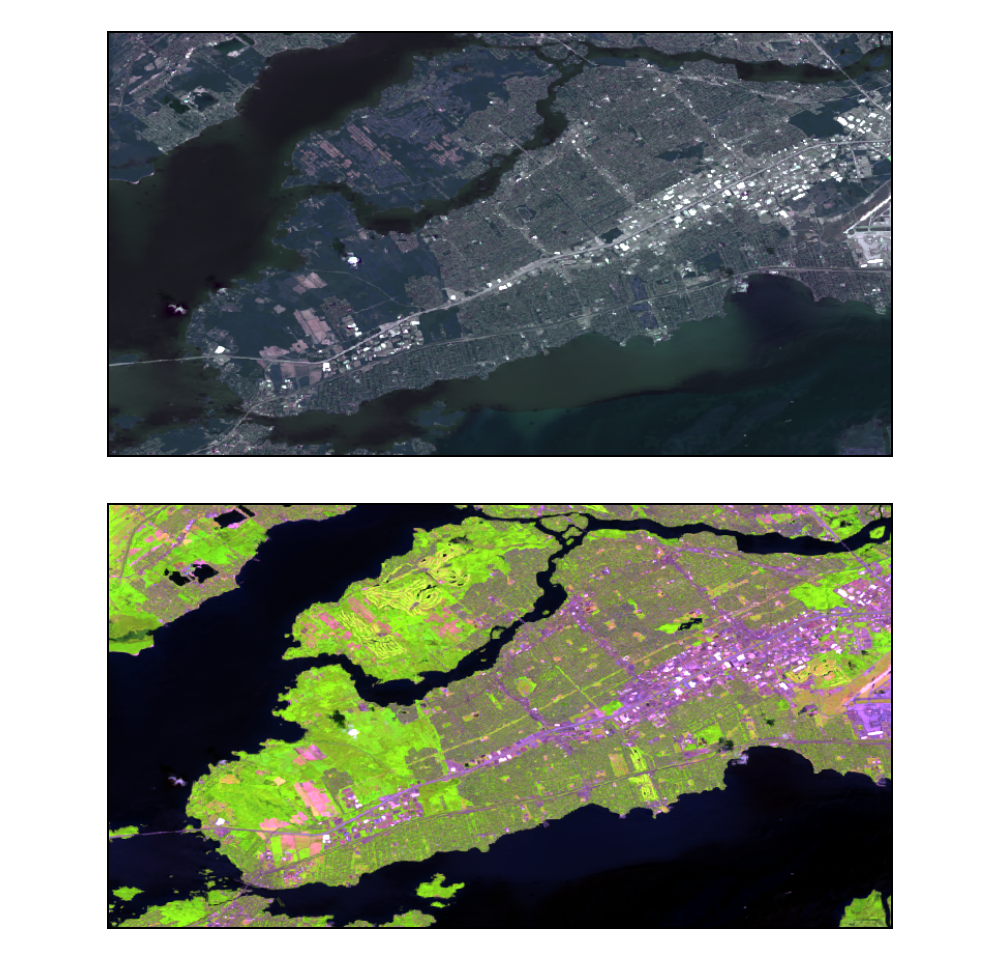
\includegraphics{chapters/clustering_files/figure-pdf/fig-kmeans-composites-output-1.png}

}

\sidecaption{\label{fig-kmeans-composites}The Landsat 9 data are
combined into the ``Natural Color'' image, in which the red, green, and
blue bands are mapped to their respective channels (left). The other
composites is a 6-5-4 image meant to show differences between urban
areas, vegetations, and crops. Note that the true-color composite is
slightly distored compared to the colors of the landscape we expect;
this is because natural colors are difficult to reproduce accurately.}

\end{figure}%

In Figure~\ref{fig-kmeans-composites}, we compare the natural color
reconstruction (top) to a false color composite. All of the panels in
Figure~\ref{fig-kmeans-composites} represent the same physical place at
the same moment in time; but through them, we are looking at this place
with very different purposes. This is not an idle observation, but a
core notion in data science: \emph{what we measure defines what we can
see}. In order to tell something ecologically meaningful about this
place, we need to look at it in the ``right'' way. Of course, although
remote sensing offers a promising way to collect data for biodiversity
monitoring at scale (Gonzalez \emph{et al.} 2023), there is no guarantee
that it will be the right approach for all problems. More (fancier) data
is not necessarily right for all problems.

\marginnote{\begin{footnotesize}

We will revisit the issue of variable selection and feature engineering
in Chapter~\ref{sec-variable-selection}.

\end{footnotesize}}

So far, we have looked at this area by combining the raw data. Depending
on the question we have in mind, they may not be the \emph{right} data.
In fact, they may not hold information that is relevant to our question
\emph{at all}; or worse, they can hold more noise than signal. The area
we will work on in this chapter is a very small crop of a Landsat 9
scene, taken on path 14 and row 28, early in late June 2023. It shows
the western tip of the island of Montréal, as well as Lake Saint-Louis
to the south (not actually a lake), Lake Deux-Montages to the north (not
actually a lake either), and a small part of Oka national park. This is
an interesting area because it has a high variety of environments: large
bodies of water, forested areas (bright green in the composite), densely
urbanized places (bright purple and white in the composite), less
densely urbanized (green-brown), and cropland to the western tip of the
island.

But can we classify these different environments starting in an
ecologically relevant way? Based on our knowledge of plants, we can
start thinking about this question in a different way. Specifically,
``can we guess that a pixel contains plants?'', and ``can we guess at
how much water there is in a pixel?''. Thankfully, ecologists, whose
hobbies include (i) guesswork and (ii) plants, have ways to answer these
questions rather accurately.

One way to do this is to calculate the normalized difference vegetation
index, or NDVI (Kennedy \& Burbach 2020). NDVI is derived from the band
data (NIR - Red), and there is an adequate heuristic using it to make a
difference between vegetation, barren soil, and water. Because plants
are immediately tied to water, we can also consider the NDWI (water;
Green - NIR) and NDMI (moisture; NIR - SWIR1) dimensions: taken
together, these information will represent every pixel in a
three-dimensional space, telling us whether there are plants (NDVI),
whether they are stressed (NDMI), and whether this pixel is a water body
(NDWI). Other commonly used indices based on Landsat 9 data include the
NBR (Normalized Burned Ratio), for which high values are suggestive of a
history of intense fire (Roy \emph{et al.} 2006 have challenged the idea
that this measure is relevant immediately post-fire), and the NDBI
(Normalized Difference Built-up Index) for urban areas.

We can look at the relationship between the NDVI and NDMI data
Figure~\ref{fig-kmeans-hexbin}. For example, NDMI values around -0.1 are
\href{https://eos.com/make-an-analysis/ndmi/}{low-canopy cover with low
water stress}; NDVI values from 0.2 to 0.5 are good candidates for
moderately dense crops. Notice that there is a strong (linear)
relationship between NDVI and NDMI. Indeed, none of these indices are
really independent; this implies that they are likely to be more
informative taken together than when looking at them one at a time
(Zheng \emph{et al.} 2021). Indeed, urban area tend to have high values
of the NDWI, which makes the specific task of looking for swimming pools
(for mosquito control) more challenging than it sounds (McFeeters 2013).

\begin{figure}[bt]

\centering{

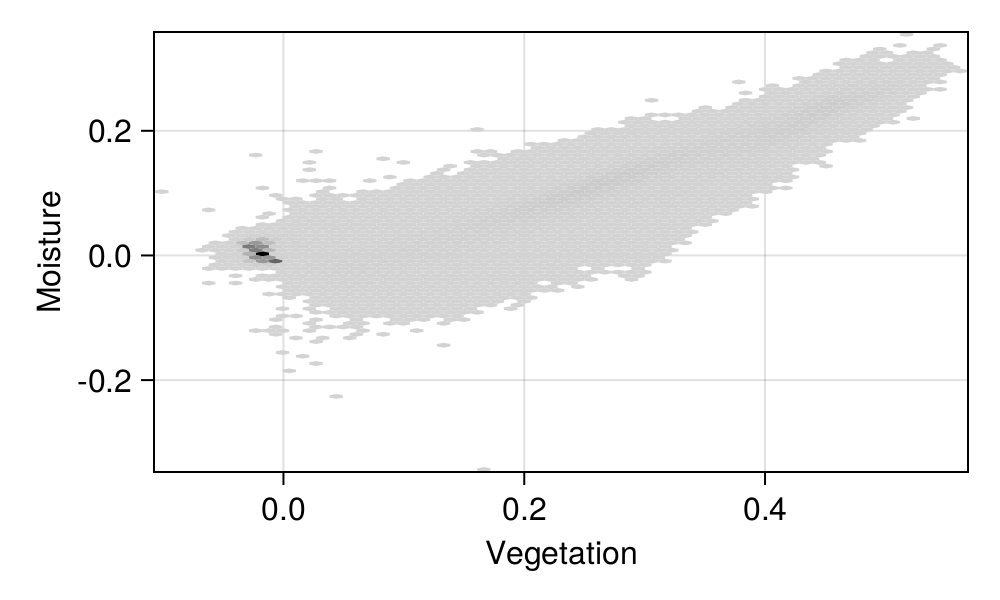
\includegraphics{chapters/clustering_files/figure-pdf/fig-kmeans-hexbin-output-1.png}

}

\sidecaption{\label{fig-kmeans-hexbin}The pixels acquired from Landsat 9
exist in a space with many different dimensions (one for each band).
Because we are interested in a landscape classification based on water
and vegetation data, we use the NDVI, NDMI, and NDWI combinations of
bands. These are \emph{derived} data, and represent the creation of new
features from the raw data. Darker colors indicate more pixels in this
bin.}

\end{figure}%

By picking these four transformed values, instead of simply looking at
the clustering of all the bands in the raw data, we are starting to
refine what the algorithm sees, through the lens of what we know is
important about the system. With these data in hands, we can start
building a classification algorithm.

\section{\texorpdfstring{The theory behind \emph{k}-means
clustering}{The theory behind k-means clustering}}\label{the-theory-behind-k-means-clustering}

In order to understand the theory underlying \emph{k}-means, we will
work backwards from its output. As a method for clustering,
\emph{k}-means will return a vector of \emph{class memberships}, which
is to say, a list that maps each observation (pixel, in our case) to a
class (tentatively, a cohesive landscape unit). What this means is that
\emph{k}-means is a transformation, taking as its input a vector with
three dimensions (NDVI, NDMI, NDWI), and returning a scalar (an integer,
even!), giving the class to which this pixel belongs. Pixels only
belongs to one class. These are the input and output of our blackbox,
and now we can start figuring out its internals.

\subsection{Inputs and parameters}\label{inputs-and-parameters}

\marginnote{\begin{footnotesize}

Throughout this book, we will use \(\mathbf{X}\) to note the matrix of
features, and \(\mathbf{y}\) to note the vector of labels. Instances are
columns of the features matrix, noted \(\mathbf{x}_i\).

\end{footnotesize}}

In \emph{k}-means, a set of observations \(\mathbf{x}_i\) are assigned
to a set of classes \(\mathbf{C}\), also called the clusters. All
\(\mathbf{x}_i\) are vectors with the same dimension (we will call it
\(f\), for \emph{features}), and we can think of our observations as a
matrix of features \(\mathbf{X}\) of size \((f, n)\), with \(f\)
features and \(n\) observations (the columns of this matrix).

The number of classes of \(\mathbf{C}\) is \(|\mathbf{C}| = k\), and
\(k\) is an hyper-parameter of the model, as it needs to fixed before we
start running the algorithm. Each class is defined by its centroid, a
vector \(\mathbf{c}\) with \(f\) dimensions (\emph{i.e.} the centroid
corresponds to a potential ``idealized'' observation of this class in
the space of the features), which \emph{k}-means progressively refines.

\subsection{Assigning instances to
classes}\label{assigning-instances-to-classes}

\marginnote{\begin{footnotesize}

Of course, the correct distance measure to use depends on what is
appropriate for the data!

\end{footnotesize}}

Instances are assigned to the class for which the distance between
themselves and the centroid of this class is lower than the distance
between themselves and the centroid of any other class. To phrase it
differently, the class membership of an instance \(\mathbf{x}_i\) is
given by

\begin{equation}\phantomsection\label{eq-clustering-onepoint}{
\text{argmin}_j \left\|\mathbf{x}_i-\mathbf{c}_j\right\|_2 \,,
}\end{equation}

which is the value of \(j\) that minimizes the \(L^2\) norm
(\(\|\cdot\|_2\), the Euclidean distance) between the instance and the
centroid; \(\text{argmin}_j\) is the function returning the value of
\(j\) that minimizes its argument. For example,
\(\text{argmin}(0.2,0.8,0.0)\) is \(3\), as the third argument is the
smallest. There exists an \(\text{argmax}\) function, which works in the
same way.

\subsection{Optimizing the centroids}\label{optimizing-the-centroids}

Of course, what we really care about is the assignment of \emph{all}
instances to the classes. For this reason, the configuration (the
disposition of the centroids) that solves our specific problem is the
one that leads to the lowest possible variance within the clusters. As
it turns out, it is not that difficult to go from
Equation~\ref{eq-clustering-onepoint} to a solution for the entire
problem: we simply have to sum over all points!

This leads to a measure of the variance, which we want to minimize,
expressed as

\begin{equation}\phantomsection\label{eq-clustering-variance}{
\sum_{i=1}^k \sum_{\mathbf{x}\in \mathbf{C}_i} \|\mathbf{x} - \mathbf{c}_i\|_2 \,.
}\end{equation}

The part that is non-trivial is now to decide on the value of
\(\mathbf{c}\) for each class. This is the heart of the \emph{k}-means
algorithm. From Equation~\ref{eq-clustering-onepoint}, we have a
criteria to decide to which class each instance belongs. Of course,
there is nothing that prevents us from using this in the opposite
direction, to define the instance by the points that form it! In this
approach, the membership of class \(\mathbf{C}_j\) is the list of points
that satisfy the condition in Equation~\ref{eq-clustering-onepoint}. But
there is no guarantee that the \emph{current} position of
\(\mathbf{c}_j\) in the middle of all of these points is optimal,
\emph{i.e.} that it minimizes the within-class variance.

This is easily achieved, however. To ensure that this is the case, we
can re-define the value of \(\mathbf{c}_j\) as

\begin{equation}\phantomsection\label{eq-clustering-centroid-update}{
\mathbf{c}_j = \frac{1}{|\mathbf{C}_j|}\sum\mathbf{C}_j \,,
}\end{equation}

where \(|\cdot|\) is the cardinality of (number of istances in)
\(\mathbf{C}_j\), and \(\sum \mathbf{C}_j\) is the sum of each feature
in \(\mathbf{C}_j\). To put it plainly: we update the centroid of
\(\mathbf{C}_j\) so that it takes, for each feature, the average value
of all the instances that form \(\mathbf{C}_j\).

\subsection{Updating the classes}\label{updating-the-classes}

\marginnote{\begin{footnotesize}

Repeating a step multiple times in a row is called an iterative process,
and we will see a \emph{lot} of them.

\end{footnotesize}}

Once we have applied Equation~\ref{eq-clustering-centroid-update} to all
classes, there is a good chance that we have moved the centroids in a
way that moved them away from some of the points, and closer to others:
the membership of the instances has likely changed. Therefore, we need
to re-start the process again, in an iterative way.

But until when?

Finding the optimal solution for a set of points is an NP-hard problem
(Aloise \emph{et al.} 2009), which means that we will need to rely on a
little bit of luck, or a whole lot of time. The simplest way to deal
with iterative processes is to let them run for a long time, as after a
little while they should converge onto an optimum (here, a set of
centroids for which the variance is as good as it gets), and hope that
this optimum is \emph{global} and not \emph{local}.

A global optimum is easy to define: it is the state of the solution that
gives the best possible result. For this specific problem, a global
optimum means that there are no other combinations of centroids that
give a lower variance. A local optimum is a little bit more subtle: it
means that we have found a combination of centroids that we cannot
improve without first making the variance worse. Because the algorithm
as we have introduced it in the previous sections is \emph{greedy}, in
that it makes the moves that give the best short-term improvement, it
will not provide a solution that temporarily makes the variance higher,
and therefore is susceptible to being trapped in a local optimum.

In order to get the best possible solution, it is therefore common to
run \emph{k}-means multiple times for a given \(k\), and to pick the
positions of the centroids that give the best overall fit.

\subsection{Identification of the optimal number of
clusters}\label{sec-clustering-optimality}

One question that is left un-answered is the value of \(k\). How do we
decide on the number of clusters?

There are two solutions here. One is to have an \emph{a priori}
knowledge of the number of classes. For example, if the purpose of
clustering is to create groups for some specific task, there might be an
upper/lower bound to the number of tasks you are willing to consider.
The other solution is to run the algorithm in a way that optimizes the
number of clusters for us.

This second solution turns out to be rather simple with \emph{k}-means.
We need to change the value of \(k\), run it on the same dataset several
times, and then pick the solution that was \emph{optimal}. But this is
not trivial. Simply using Equation~\ref{eq-clustering-variance} would
lead to always preferring many clusters. After all, each point in its
own cluster would get a pretty low variance!

For this reason, we use measures of optimality that are a little more
refined. One of them is the Davies \& Bouldin (1979) method, which is
built around a simple idea: an assignment of instances to clusters is
good if the instances within a cluster are not too far away from the
centroids, and the centroids are as far away from one another as
possible.

The Davies-Bouldin measure is striking in its simplicity. From a series
of points and their assigned clusters, we only need to compute two
things. The first is a vector \(\mathbf{s}\), which holds the average
distance between the points and their centroids (this is the
\(\left\|\mathbf{x}_i-\mathbf{c}_j\right\|_2\) term in
Equation~\ref{eq-clustering-onepoint}, so this measure still relates
directly to the variance); the second is a matrix \(\mathbf{M}\), which
measures the distances \emph{between} the centroids.

These two information are combined in a matrix \(\mathbf{R}\), wherein
\(\mathbf{R}_{ij} = (s_i + s_j)/\mathbf{M}_{ij}\). The interpretation of
this term is quite simply: is the average distance \emph{within}
clusters \(i\) and \(j\) much larger compared to the distance
\emph{between} these clusters. This is, in a sense, a measure of the
stress that these two clusters impose on the entire system. In order to
turn this matrix into a single value, we calculate the maximum value
(ignoring the diagonal!) for each row: this is a measure of the
\emph{maximal} amount of stress in which a cluster is involved. By
averaging these values across all clusters, we have a measure of the
quality of the assignment, that can be compared for multiple values of
\(k\).

Note that this approach protects us against the
each-point-in-its-cluster situation: in this scenario, the distance
between clusters would decrease really rapidly, meaning that the values
in \(\mathbf{R}\) would \emph{increase}; the Davies-Bouldin measure
indicates a better clustering when the values are \emph{lower}.

\marginnote{\begin{footnotesize}

In fact, there is very little enumeration of techniques in this book.
The important point is to understand how all of the pieces fit together,
not to make a census of all possible pieces.

\end{footnotesize}}

There are alternatives to this method, including silhouettes (Rousseeuw
1987) and the technique of Dunn (1974). The question of optimizing the
number of clusters goes back several decades (Thorndike 1953), and it
still actively studied. What matter is less to give a comprehensive
overview of all the measures: the message here is to pick one that works
(and can be justified) for your specific problem!

\section{Application: optimal clustering of the satellite image
data}\label{application-optimal-clustering-of-the-satellite-image-data}

\subsection{Initial run}\label{sec-kmeans-initial}

Before we do anything else, we need to run our algorithm with a random
pick of hyper-parameters, in order to get a sense of how hard the task
ahead is. In this case, using \(k = 3\), we get the results presented in
Figure~\ref{fig-kmeans-initial-landscape}.

\begin{figure}[bt]

\centering{

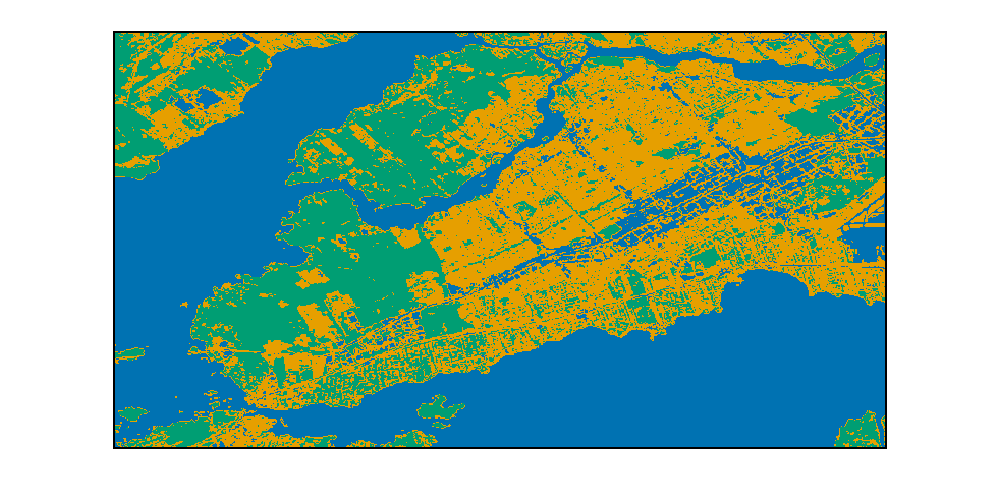
\includegraphics{chapters/clustering_files/figure-pdf/fig-kmeans-initial-landscape-output-1.png}

}

\sidecaption{\label{fig-kmeans-initial-landscape}After iterating the
\emph{k}-means algorithm, we obtain a classification for every pixel in
the landscape. This classification is based on the values of NDVI, NDMI,
and NDWI indices, and therefore groups pixels based on specific
assumptions about vegetation and stress. This clustering was produced
using \(k=3\), \emph{i.e.} we want to see what the landscape would look
like when divided into three categories.}

\end{figure}%

\marginnote{\begin{footnotesize}

In fact, take some time to think about how you would use \(k\)-means to
come up with a way to remove pixels with only water from this image!

\end{footnotesize}}

It is always a good idea to look at the first results and state the
obvious. Here, for example, we can say that water is easy to identify.
In fact, removing open water pixels from images is an interesting image
analysis challenge (Mondejar \& Tongco 2019), and because we used an
index that specifically identifies water bodies (NDWI), it is not
surprising that there is an entire cluster that seems to be associated
with water. But if we take a better look, it appears that there groups
of pixels that represent dense urban areas that are classified with the
water pixels. When looking at the landscape in a space with three
dimensions, it looks like separating densely built-up environment and
water is difficult.

This might seem like an idle observation, but this is not the case! It
means that when working on vegetation-related questions, we will likely
need at least one cluster for water, and one cluster for built-up areas.
This is helpful information, because we can already think about how many
classes of vegetation we are willing to accept, and add (at least) two
clusters to capture other types of cover.

\subsection{Optimal number of pixels}\label{optimal-number-of-pixels}

\marginnote{\begin{footnotesize}

We will revisit the issue of tuning the hyper-parameters in more depth
in Chapter~\ref{sec-tuning}.

\end{footnotesize}}

In order to produce Figure~\ref{fig-kmeans-initial-landscape}, we had to
guess at a number of classes we wanted to split the landscape into. This
introduces two important steps in coming up with a model: starting with
initial parameters in order to iterate rapidly, and then refining these
parameters to deliver a model that is fit for purpose. Our discussion in
Section~\ref{sec-kmeans-initial}, where we concluded that we needed to
keep (maybe) two classes for water and built-up is not really
satisfying, as we do not yet have a benchmark to evaluate the correct
value of \(k\); we know that it is more than 3, but how much more?

We will now change the values of \(k\) and use the Davies \& Bouldin
(1979) measure introduced in Section~\ref{sec-clustering-optimality} to
identify the optimal value of \(k\). The results are presented in
Figure~\ref{fig-kmeans-tuning}. Note that we only explore
\(k \in [3, 10]\). More than 8 categories is probably not very
actionable, and therefore we can make the decision to only look at this
range of parameters. Sometimes (always!) the best solution is the one
that gets your job done.

\begin{figure}[bt]

\centering{

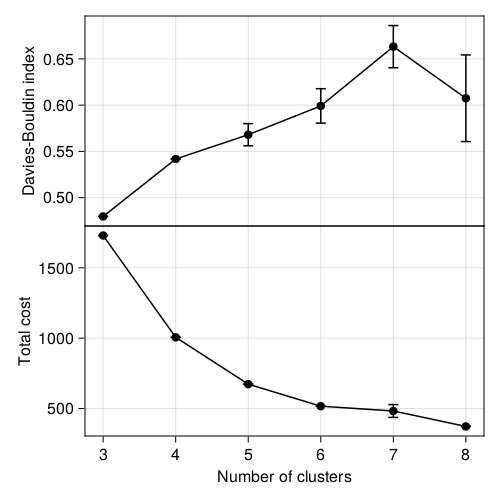
\includegraphics{chapters/clustering_files/figure-pdf/fig-kmeans-tuning-output-1.png}

}

\sidecaption{\label{fig-kmeans-tuning}Results of running the
\emph{k}-means algorithm ten times for each number of clusters between 3
and 8. The average Davies-Bouldin and cost are reported, as well as the
standard deviation. As expected, the total cost decreases with more
clusters, but this is not necessarily the sign of a better clustering.}

\end{figure}%

There are two interesting things in Figure~\ref{fig-kmeans-tuning}.
First, note that for \(k=\{3,4\}\), there is almost no dispersal: all of
the assignments have the exact same score, which is unlikely to happen
except if the assignments are the same every time! This is a good sign,
and, anecdotally, something that might suggest a really information
separation of the points. Second, \(k = 3\) has by far the lowest
Davies-Bouldin index of all values we tried, and is therefore strongly
suggestive of an optimal hyper-parameter. But in
Figure~\ref{fig-kmeans-initial-landscape}, we already established that
one of these clusters was capturing \emph{both} water and built-up
environments, so although it may look better from a quantitative point
of view, it is not an ideal solution \emph{for the specific problem we
have}.

In this specific case, it makers very little sense \emph{not} to use
\(k = 4\) or \(k = 5\). They have about the same performance, but this
gives us potentially more classes that are neither water nor built-up.
This image is one of many cases where it is acceptable to sacrifice a
little bit of optimality in order to present more actionable
information. Based on the results in this section, we will pick the
largest possible \(k\) that does not lead to a drop in performance,
which in our case is \(k=5\).

\subsection{Clustering with optimal number of
classes}\label{clustering-with-optimal-number-of-classes}

The clustering of pixels using \(k = 5\) is presented in
Figure~\ref{fig-kmeans-optimal-landscape}. Unsurprisingly,
\emph{k}-means separated the open water pixels, the dense urban areas,
as well as the more forested/green areas. Now is a good idea to start
thinking about what is representative of these clusters: one is
associated with very high NDWI value (these are the water pixels), and
two classes have both high NDVI and high NDMI (suggesting different
categories of vegetation).

\begin{verbatim}
┌ Warning: The clustering cost increased at iteration #37
└ @ Clustering ~/.julia/packages/Clustering/yuxBr/src/kmeans.jl:191
\end{verbatim}

\begin{figure}[bt]

\centering{

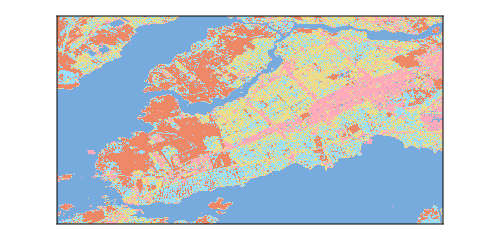
\includegraphics{chapters/clustering_files/figure-pdf/fig-kmeans-optimal-landscape-output-2.png}

}

\sidecaption{\label{fig-kmeans-optimal-landscape}Results of the
landscape clustering with k=5 clusters. This number of clusters gives us
a good separation between different groups of pixels, and seems to
capture features of the landscape as revealed with the false-color
composites.}

\end{figure}%

\marginnote{\begin{footnotesize}

We will revisit the issue of understanding how a model makes a
prediction in Chapter~\ref{sec-explanations}.

\end{footnotesize}}

The relative size of the clusters (as well as the position of their
centroids) is presented in Table~\ref{tbl-clustering-centers}. There is
a good difference in the size of the clusters, which is an important
thing to note. Indeed, a common myth about \emph{k}-means is that it
gives clusters of the same size. This ``size'' does not refer to the
cardinality of the clusters, but to the volume that they cover in the
space of the parameters. If an area of the space of parameters is more
densely packed with instances, the cluster covering the area will have
more points!

\begin{table}

\caption{\label{tbl-clustering-centers}Summary of the values for the
centers of the optimal clusters found in this image. The cover column
gives the percentage of all pixels associated to this class. The
clusters are sorted by the NDVI of their centroid.}

\centering{

\begin{longtable}[]{@{}rrrrr@{}}
\toprule\noalign{}
Cluster & Cover & NDVI & NDWI & NDMI \\
\midrule\noalign{}
\endhead
\bottomrule\noalign{}
\endlastfoot
1 & 38 & -0.018 & 0.012 & 0.006 \\
4 & 10 & 0.096 & -0.152 & 0.005 \\
3 & 19 & 0.224 & -0.262 & 0.08 \\
5 & 17 & 0.32 & -0.343 & 0.139 \\
2 & 16 & 0.439 & -0.443 & 0.223 \\
\end{longtable}

}

\end{table}%

\marginnote{\begin{footnotesize}

In fact, this behavior makes \emph{k}-means excellent at creating color
palettes from images! Cases in point,
\href{https://github.com/karthik/wesanderson}{Karthik Ram's Wes Anderson
palettes}, and \href{https://github.com/dill/beyonce}{David Lawrence
Miller's Beyoncé palettes}. Let it never again be said that ecologists
should not be trusted with machine learning methods.

\end{footnotesize}}

The area of the space of parameters covered by each cluster in
represented in Figure~\ref{fig-kmeans-clustering}, and this result is
actually not surprising, if we spend some time thinking about how
\emph{k}-means work. Because our criteria to assign a point to a cluster
is based on the being closest to its centroid than to any other
centroid, we are essentially creating Voronoi cells, with linear
boundaries between them.

By opposition to a model based on, for example, mixtures of Gaussians,
the assignment of a point to a cluster in \emph{k}-means is independent
of the current composition of the cluster (modulo the fact that the
current composition of the cluster is used to update the centroids). In
fact, this makes \emph{k}-means closer to (or at least most efficient
as) a method for quantization (Gray 1984).

\begin{figure}[bt]

\centering{

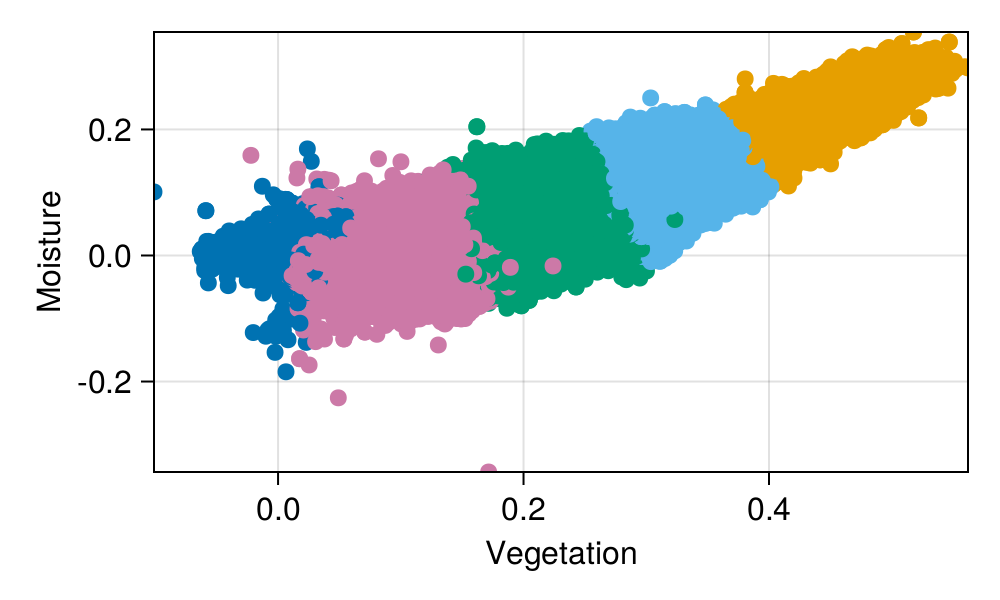
\includegraphics{chapters/clustering_files/figure-pdf/fig-kmeans-clustering-output-1.png}

}

\sidecaption{\label{fig-kmeans-clustering}Visualisation of the
clustering output as a function of the NDVI and NDMI values. Note that
the limits between the clusters are lines (planes), and that each
cluster covers about the same volume in the space of parameters.}

\end{figure}%

\section{Conclusion}\label{conclusion}

In this chapter, we have used the \emph{k}-means algorithm to create
groups in a large dataset that had no labels, \emph{i.e.} the points
were not assigned to a class. By picking the features we wanted to
cluster the point, we were able to highlight specific aspects of the
landscape. In Chapter~\ref{sec-gradientdescent}, we will start adding
labels to our data, and shift our attention from classification to
regression problems.

\bookmarksetup{startatroot}

\chapter{Gradient descent}\label{sec-gradientdescent}

As we progress into this book, the process of delivering a trained model
is going to become more and more complex. In
Chapter~\ref{sec-clustering}, we worked with a model that did not really
require training (but did require to pick the best hyper-parameter). In
this chapter, we will only increase complexity very slightly, by
considering how we can train a model when we have a reference dataset to
compare to.

Doing do will require to introduce several new concepts, and so the
``correct'' way to read this chapter is to focus on the high-level
process. The problem we will try to solve (which is introduced in
Section~\ref{sec-gradientdescent-problem}) is very simple; in fact, the
empirical data looks more fake than many simulated datasets!

\section{A digression: what is a trained
model?}\label{sec-gradientdescent-trainedmodel}

Models are data. When a model is trained, it represents a series of
measurements (its parameters), taken on a representation of the natural
world (the training data), through a specific instrument (the model
itself, see \emph{e.g.} Morrison \& Morgan 1999). A trained model is,
therefore, capturing our understanding of a specific situation we
encountered. We need to be very precise when defining what, exactly, a
model describes. In fact, we need to take a step back and try to figure
out where the model stops.

As we will see in this chapter, then in
Chapter~\ref{sec-crossvalidation}, and finally in
Chapter~\ref{sec-tuning}, the fact of training a model means that there
is a back and forth between the algorithm we train, the data we use for
training, and the criteria we set to define the performance of the
trained model. The algorithm bound to its dataset is the \emph{machine}
we train in machine learning.

Therefore, a trained model is never independent from its training data:
they describe the scope of the problem we want to address with this
model. In Chapter~\ref{sec-clustering}, we ended up with a machine (the
trained \emph{k}-means algorithm) whose parameters (the centroids of the
classes) made sense in the specific context of the training data we
used; applied to a different dataset, there are no guarantees that our
model would deliver useful information.

For the purpose of this book, we will consider that a model is trained
when we have defined the algorithm, the data, the measure through which
we will evaluate the model performance, and then measured the
performance on a dataset built specifically for this task. All of these
elements are important, as they give us the possibility to
\emph{explain} how we came up with the model, and therefore, how we made
the predictions. This is different from reasoning about why the model is
making a specific prediction (we will discuss this in
Chapter~\ref{sec-explanations}), and is more related to explaining the
process, the ``outer core'' of the model. As you read this chapter, pay
attention to these elements: what algorithm are we using, on what data,
how do we measure its performance, and how well does it perform?

\section{The problem: how many interactions in a food
web?}\label{sec-gradientdescent-problem}

One of the earliest observation that ecologists made about food webs is
that when there are more species, there are more interactions. A
remarkably insightful crowd, food web ecologists. Nevertheless, it turns
out that this apparently simple question had received a few different
answers over the years.

The initial model was proposed by Cohen \& Briand (1984): the number of
interactions \(L\) scales linearly with the number of species \(S\).
After all, we can assume that when averaging over many consumers, there
will be an average diversity of resources they consume, and so the
number of interactions could be expressed as \(L \approx b\times S\).

Not so fast, said Martinez (1992). When we start looking a food webs
with more species, the increase of \(L\) with regards to \(S\) is
superlinear. Thinking in ecological terms, maybe we can argue that
consumers are flexible, and that instead of sampling a set number of
resources, they will sample a set proportion of the number of
consumer-resource combinations (of which there are \(S^2\)). In this
interpretation, \(L \approx b\times S^2\).

But the square term can be relaxed; and there is no reason not to assume
a power law, with \(L\approx b\times S^a\). This last formulation has
long been accepted as the most workable one, because it is possible to
approximate values of its parameters using other ecological processes
(Brose \emph{et al.} 2004).

The ``reality'' (\emph{i.e.} the relationship between \(S\) and \(L\)
that correctly accounts for ecological constraints, and fit the data as
closely as possible) is a little bit different than this formula
(MacDonald \emph{et al.} 2020). But for the purpose of this chapter,
figuring out the values of \(a\) and \(b\) from empirical data is a very
instructive exercise.

In Figure~\ref{fig-gradient-data}, we can check that there is a linear
relationship between the natural log of the number of species and the
natural log of the number of links. This is not surprising! If we assume
that \(L \approx b\times S^a\), then we can take the log of both sides,
and we get
\(\text{log}\, L \approx a \times \text{log}\, S + \text{log}\,b\). This
is linear model, and so we can estimate its parameters using linear
regression!

\begin{figure}[bt]

\centering{

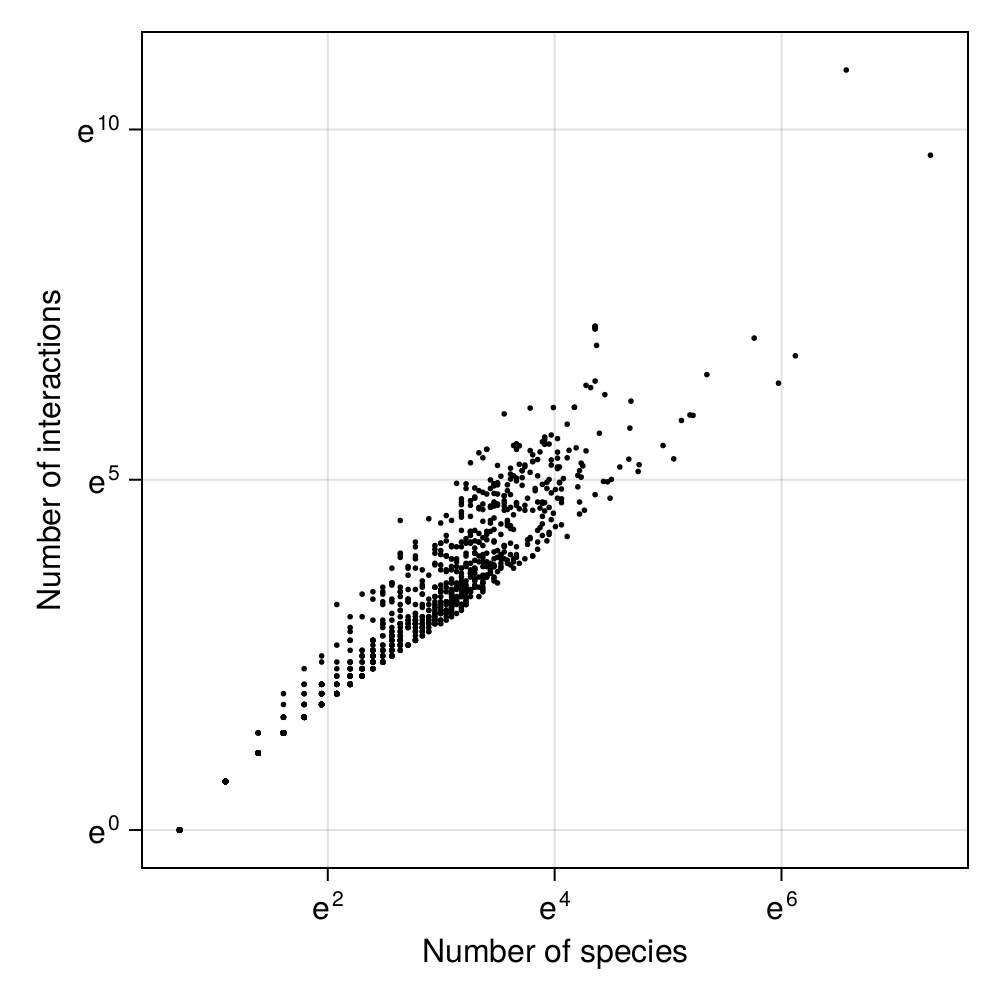
\includegraphics{chapters/gradientdescent_files/figure-pdf/fig-gradient-data-output-1.png}

}

\sidecaption{\label{fig-gradient-data}We have assumed that the
relationship between \(L\) and \(S\) could be represented by
\(L \approx b\times S^a\), which gave us a reason to take the natural
log of both variables. On this figure, we see that the relationship
between the logs look linear, which means that linear regression has a
good chance of estimating the values of the parameters.}

\end{figure}%

\section{Gradient descent}\label{sec-gradientdescent-explanation}

Gradient descent is built around a remarkably simple intuition: knowing
the formula that gives rise to our prediction, and the value of the
error we made for each point, we can take the derivative of the error
with regards to each parameter, and this tells us how much this
parameter contributed to the error. Because we are taking the
derivative, we can futher know whether to increase, or decrease, the
value of the parameter in order to make a smaller error next time.

In this section, we will use linear regression as an example, because it
is the model we have decided to use when exploring our ecological
problem in Section~\ref{sec-gradientdescent-problem}, and because it is
suitably simple to keep track of everything when writing down the
gradient by hand.

Before we start assembling the different pieces, we need to decide what
our model is. We have settled on a linear model, which will have the
form \(\hat y = m\times x + b\). The little hat on \(\hat y\) indicates
that this is a prediction. The input of this model is \(x\), and its
parameters are \(m\) (the slope) and \(b\) (the intercept). Using the
notation we adopted in Section~\ref{sec-gradientdescent-problem}, this
would be \(\hat l = a \times s + b\), with \(l = \text{log} L\) and
\(s = \text{log} S\).

\subsection{Defining the loss
function}\label{sec-gradientdescent-lossfunctions}

The loss function is an important concept for anyone attempting to
compare predictions to outcomes: it quantifies how far away an ensemble
of predictions is from a benchmark of known cases. There are many loss
functions we can use, and we will indeed use a few different ones in
this book. But for now, we will start with a very general understanding
of what these functions \emph{do}.

Think of prediction as throwing a series of ten darts on ten different
boards. In this case, we know what the correct outcome is (the center of
the board, I assume, although I can be mistaken since I have only played
darts once, and lost). A cost function would be any mathematical
function that compares the position of each dart on each board, the
position of the correct event, and returns a score that informs us about
how poorly our prediction lines up with the reality.

In the above example, you may be tempted to say that we can take the
Euclidean distance of each dart to the center of each board, in order to
know, for each point, how far away we landed. Because there are several
boards, and because we may want to vary the number of boards while still
retaining the ability to compare our performances, we would then take
the average of these measures.

We will note the position of our dart as being \(\hat y\), the position
of the center as being \(y\) (we will call this the \emph{ground
truth}), and the number of attempts \(n\), and so we can write our loss
function as

\begin{equation}\phantomsection\label{eq-loss-mse}{
\frac{1}{n}\sum_{i=1}^{n}(y_i - \hat y_i)^2
}\end{equation}

\marginnote{\begin{footnotesize}

In data science, things often have multiple names. This is true of loss
functions, and this will be even more true on other things later.

\end{footnotesize}}

This loss function is usually called the MSE (Mean Standard Error), or
L2 loss, or the quadratic loss, because the paths to machine learning
terminology are many. This is a good example of a loss function for
regression (and we will discuss loss functions for classification later
in this book). There are alternative loss functions to use for
regression problems in Table~\ref{tbl-gradientdescent-regressionloss}.

\begin{longtable}[]{@{}
  >{\raggedright\arraybackslash}p{(\columnwidth - 4\tabcolsep) * \real{0.4722}}
  >{\raggedright\arraybackslash}p{(\columnwidth - 4\tabcolsep) * \real{0.2639}}
  >{\raggedright\arraybackslash}p{(\columnwidth - 4\tabcolsep) * \real{0.2639}}@{}}
\caption{List of common loss functions for regression problems
\{tbl-colwidths=\textquotesingle{[}25,25,50{]}\textquotesingle\}}\label{tbl-gradientdescent-regressionloss}\tabularnewline
\toprule\noalign{}
\begin{minipage}[b]{\linewidth}\raggedright
Measure
\end{minipage} & \begin{minipage}[b]{\linewidth}\raggedright
Expression
\end{minipage} & \begin{minipage}[b]{\linewidth}\raggedright
Remarks
\end{minipage} \\
\midrule\noalign{}
\endfirsthead
\toprule\noalign{}
\begin{minipage}[b]{\linewidth}\raggedright
Measure
\end{minipage} & \begin{minipage}[b]{\linewidth}\raggedright
Expression
\end{minipage} & \begin{minipage}[b]{\linewidth}\raggedright
Remarks
\end{minipage} \\
\midrule\noalign{}
\endhead
\bottomrule\noalign{}
\endlastfoot
Mean Squared Error (MSE, L2) &
\(\frac{1}{n}\sum_{i=1}^{n}\left(y_i - \hat y_i\right)^2\) & Large
errors are (proportionally) more penalized because of the squaring \\
Mean Absolute Error (MAE, L1) &
\(\frac{1}{n}\sum_{i=1}^{n}\|y_i - \hat y_i\|\) & Error measured in the
units of the response variable \\
Root Mean Square Error (RMSE) & \(\sqrt{\text{MSE}}\) & Error measured
in the units of the response variable \\
Mean Bias Error &
\(\frac{1}{n}\sum_{i=1}^{n}\left(y_i - \hat y_i\right)\) & Errors
\emph{can} cancel out, but this can be used as a measure of
positive/negative bias \\
\end{longtable}

Throughout this chapter, we will use the L2 loss
(Equation~\ref{eq-loss-mse}), because it has \emph{really} nice
properties when it comes to taking derivatives, which we will do a lot
of. In the case of a linear model, we can rewrite
Equation~\ref{eq-loss-mse} as

\begin{equation}\phantomsection\label{eq-loss-withmodel}{
f = \frac{1}{n}\sum\left(y_i - m\times x_i - b\right)^2
}\end{equation}

There is an important change in Equation~\ref{eq-loss-withmodel}: we
have replaced the prediction \(\hat y_i\) with a term that is a function
of the predictor \(x_i\) and the model parameters: this means that we
can calculate the value of the loss as a function of a pair of values
\((x_i, y_i)\), and the model parameters.

\subsection{Calculating the
gradient}\label{sec-gradientdescent-gradient}

With the loss function corresponding to our problem in hands
(Equation~\ref{eq-loss-withmodel}), we can calculate the gradient. Given
a function that is scalar-valued (it returns a single value), taking
several variables, that is differentiable, the gradient of this function
is a vector-valued (it returns a vector) function; when evaluated at a
specific point, this vectors indicates both the direction and the rate
of fastest increase, which is to say the direction in which the function
increases away from the point, and how fast it moves.

We can re-state this definition using the terms of the problem we want
to solve. At a point \(p = [m\quad b]^\top\), the gradient \(\nabla f\)
of \(f\) is given by:

\begin{equation}\phantomsection\label{eq-gradientdescent-gradientfull}{
\nabla f\left(
p
\right) = 
\begin{bmatrix}
\frac{\partial f}{\partial m}(p) \\
\frac{\partial f}{\partial b}(p)
\end{bmatrix}\,.
}\end{equation}

This indicates how changes in \(m\) and \(b\) will \emph{increase} the
error. In order to have a more explicit formulation, all we have to do
is figure out an expression for both of the partial derivatives. In
practice, we can let auto-differentiation software calculate the
gradient for us (Innes 2018); these packages are now advanced enough
that they can take the gradient of code directly.

Solving \((\partial f / \partial m)(p)\) and
\((\partial f / \partial c)(p)\) is easy enough:

\begin{equation}\phantomsection\label{eq-gradientdescent-gradientexplicit}{
\nabla f\left(
p
\right) = 
\begin{bmatrix}
-\frac{2}{n}\sum \left[x_i \times (y_i - m\times x_i - b)\right] \\
-\frac{2}{n}\sum \left(y_i - m\times x_i - b\right)
\end{bmatrix}\,.
}\end{equation}

Note that both of these partial derivatives have a term in \(2n^{-1}\).
Getting rid of the \(2\) in front is very straightforward! We can modify
Equation~\ref{eq-loss-withmodel} to divide by \(2n\) instead of \(n\).
This modified loss function retains the important characteristics: it
increases when the prediction gets worse, and it allows comparing the
loss with different numbers of points. As with many steps in the model
training process, it is important to think about \emph{why} we are doing
certain things, as this can enable us to make some slight changes to
facilitate the analysis.

With the gradient written down in
Equation~\ref{eq-gradientdescent-gradientexplicit}, we can now think
about what it means to \emph{descend} the gradient.

\subsection{Descending the gradient}\label{descending-the-gradient}

Recall from Section~\ref{sec-gradientdescent-gradient} that the gradient
measures how far we \emph{increase} the function of which we are taking
the gradient. Therefore, it measures how much each parameter contributes
to the loss value. Our working definition for a trained model is ``one
that has little loss'', and so in an ideal world, we could find a point
\(p\) for which the gradient is as small as feasible.

Because the gradient measures how far away we increase error, and
intuitive way to use it is to take steps in the \emph{opposite}
direction. In other words, we can update the value of our parameters
using \(p := p - \nabla f(p)\), meaning that we subtract from the
parameter values their contribution to the overall error in the
predictions.

But, as we will discuss further in
Section~\ref{sec-gradientdescent-learningrate}, there is such a thing as
``too much learning''. For this reason, we will usually not move the
entire way, and introduce a term to regulate how much of the way we
actually want to descend the gradient. Our actual scheme to update the
parameters is

\begin{equation}\phantomsection\label{eq-gradientdescent-loop}{
p := p - \eta\times \nabla f(p) \,.
}\end{equation}

This formula can be \emph{iterated}: with each successive iteration, it
will get us closer to the optimal value of \(p\), which is to say the
combination of \(m\) and \(b\) that minimizes the loss.

\subsection{A note on the learning
rate}\label{sec-gradientdescent-learningrate}

The error we can make on the first iteration will depend on the value of
our initial pick of parameters. If we are \emph{way off}, especially if
we did not re-scale our predictors and responses, this error can get
very large. And if we make a very large error, we will have a very large
gradient, and we will end up making very big steps when we update the
parameter values. There is a real risk to end up over-compensating, and
correcting the parameters too much.

In order to protect against this, in reality, we update the gradient
only a little, where the value of ``a little'' is determined by an
hyper-parameter called the \emph{learning rate}, which we noted
\(\eta\). This value will be very small (much less than one). Picking
the correct learning rate is not simply a way to ensure that we get
correct results (though that is always a nice bonus), but can be a way
to ensure that we get results \emph{at all}. The representation of
numbers in a computer's memory is tricky, and it is possible to create
an overflow: a number so large it does not fit within 64 (or 32, or 16,
or however many we are using) bits of memory.

The conservative solution of using the smallest possible learning rate
is not really effective, either. If we almost do not update our
parameters at every epoch, then we will take almost forever to converge
on the correct parameters. Figuring out the learning rate is an example
of hyper-parameter tuning, which we will get back to later in this book.

\section{Application: how many links are in a food
web?}\label{sec-gradientdescent-application}

We will not get back to the problem exposed in
Figure~\ref{fig-gradient-data}, and use gradient descent to fit the
parameters of the model defined as
\(\hat y \approx \beta_0 + \beta_1 \times x\), where, using the notation
introduced in Section~\ref{sec-gradientdescent-problem}, \(\hat y\) is
the natural log of the number of interactions (what we want to predict),
\(x\) is the natural log of the species richness (our predictor), and
\(\beta_0\) and \(\beta_1\) are the parameters of the model.

\subsection{The things we won't do}\label{the-things-we-wont-do}

At this point, we could decide that it is a good idea to transform our
predictor and our response, for example using the z-score. But this is
not really required here; we know that our model will give results that
make sense in the units of species and interactions (after dealing with
the natural log, of course). In addition, as we will see in
Chapter~\ref{sec-leakage}, applying a transformation to the data too
soon can be a dangerous thing. We will have to live with raw features
for a few more chapters.

In order to get a sense of the performance of our model, we will remove
some of the data, meaning that the model will not learn on these data
points. We will get back to this practice (cross-validation) in a lot
more details in Chapter~\ref{sec-crossvalidation}, but for now it is
enough to say that we hide 20\% of the dataset, and we will use them to
evaluate how good the model is as it trains. The point of this chapter
is not to think too deeply about cross-validation, but simply to develop
intuitions about the way a machine learns.

\subsection{Starting the learning
process}\label{starting-the-learning-process}

In order to start the gradient descent process, we need to decide on an
initial value of the parameters. There are many ways to do it. We could
work our way from our knowledge of the system; for example \(b < 1\) and
\(a = 2\) would fit relatively well with early results in the food web
literature. Or we could draw a pair of values \((a, b)\) at random.
Looking at Figure~\ref{fig-gradient-data}, it is clear that our problem
is remarkably simple, and so presumably either solution would work.

\subsection{Stopping the learning
process}\label{stopping-the-learning-process}

The gradient descent algorithm is entirely contained in
Equation~\ref{eq-gradientdescent-loop} , and so we only need to iterate
several times to optimize the parameters. How long we need to run the
algorithm for depends on a variety of factors, including our learning
rate (slow learning requires more time!), our constraints in terms of
computing time, but also how good we need to model to be.

\marginnote{\begin{footnotesize}

The number of iterations over which we train the model is usually called
the number of epochs, and is an hyper-parameter of the model.

\end{footnotesize}}

One usual approach is to decide on a number of iterations (we need to
start somewhere), and to check how rapidly the model seems to settle on
a series of parameters. But more than this, we also need to ensure that
our model is not learning \emph{too much} from the data. This would
result in over-fitting, in which the models gets better on the data we
used to train it, and worse on the data we kept hidden from the
training! In Table~\ref{tbl-gradient-attempt-one}, we present the RMSE
loss for the training and testing datasets, as well as the current
estimates of the values of the parameters of the linear model.

\begin{table}

\caption{\label{tbl-gradient-attempt-one}This table shows the change in
the model, as measured by the loss and by the estimates of the
parameters, after an increasing amount of training epochs. The loss
drops sharply in the first 500 iterations, but even after 20000
iterations, there are still some changes in the values of the
parameters.}

\centering{

\begin{longtable}[]{@{}rrrrr@{}}
\toprule\noalign{}
Step & Loss (training) & Loss (testing) & β₀ & β₁ \\
\midrule\noalign{}
\endhead
\bottomrule\noalign{}
\endlastfoot
1 & 3.92114 & 3.18785 & 0.4 & 0.2 \\
10 & 2.99934 & 2.3914 & 0.487395 & 0.226696 \\
30 & 1.72775 & 1.31211 & 0.640263 & 0.271814 \\
100 & 0.536207 & 0.373075 & 0.907004 & 0.337644 \\
300 & 0.392477 & 0.308264 & 1.03855 & 0.311011 \\
1000 & 0.326848 & 0.253939 & 1.11195 & 0.110083 \\
3000 & 0.225623 & 0.167897 & 1.25704 & -0.311373 \\
10000 & 0.164974 & 0.119597 & 1.4487 & -0.868105 \\
20000 & 0.162808 & 0.118899 & 1.48864 & -0.984121 \\
\end{longtable}

}

\end{table}%

In order to protect against over-fitting, it is common to add a check to
the training loop, to say that after a minimum number of iterations has
been done, we stop the training when the loss on the testing data starts
increasing. In order to protect against very long training steps, it is
also common to set a tolerance (absolute or relative) under which we
decide that improvements to the loss are not meaningful, and which
serves as a stopping criterion for the training.

\subsection{Detecting
over-fitting}\label{sec-gradientdescent-overfitting}

As we mentioned in the previous section, one risk with training that
runs for too long is to start seeing over-fitting. The usual diagnosis
for over-fitting is an increase in the testing loss, which is to say, in
the loss measured on the data that were not used for training. In
Figure~\ref{fig-gradient-loss-comparison}, we can see that the RMSE loss
decreases at the same rate on both datasets, which indicates that the
model is learning from the data, but not to a point where its ability to
generalize suffers.

\marginnote{\begin{footnotesize}

Underfitting is also a possible scenario, where the model is \emph{not}
learning from the data, and can be detected by seeing the loss measures
remain high or even increase.

\end{footnotesize}}

\begin{figure}[bt]

\centering{

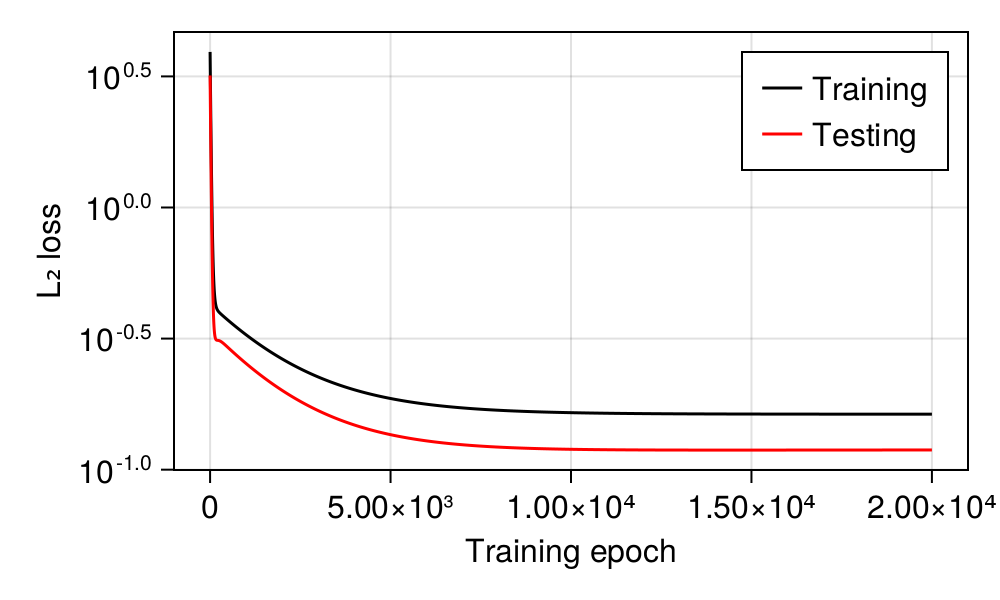
\includegraphics{chapters/gradientdescent_files/figure-pdf/fig-gradient-loss-comparison-output-1.png}

}

\sidecaption{\label{fig-gradient-loss-comparison}This figures shows the
change in the loss for the training and testing dataset. As the two
curves converge on low values at the same rate, this suggests that the
model is not over-fitting, and is therefore suitable for use.}

\end{figure}%

We are producing the loss over time figure after the training, as it is
good practice -- but as we mentioned in the previous section, it is very
common to have the training code look at the dynamics of these two
values in order to decide whether to stop the training early.

Before moving forward, let's look at
Figure~\ref{fig-gradient-loss-comparison} a little more closely. In the
first steps, the loss decreases very rapidly -- this is because we
started from a value of \(\mathbf{\beta}\) that is, presumably, far away
from the optimum, and therefore the gradient is really strong. Despite
the low learning rate, we are making long steps in the space of
parameters. After this initial rapid increase, the loss decreases much
more slowly. This, counter-intuitively, indicates that we are getting
closer to the optimum! At the exact point where \(\beta_0\) and
\(\beta_1\) optimally describe our dataset, the gradient vanishes, and
our system would stop moving. And as we get closer and closer to this
point, we are slowing down. In the next section, we will see how the
change in loss over times ties into the changes with the optimal
parameter values.

\subsection{Visualizing the learning
process}\label{visualizing-the-learning-process}

From Figure~\ref{fig-gradient-param-change}, we can see the change in
\(\beta_0\) and \(\beta_1\), as well as the movement of the current best
estimate of the parameters (right panel). The sharp decrease in loss
early in the training is specifically associated to a rapid change in
the value of \(\beta_0\). Further note that the change in parameters
values is \emph{not} monotonous! The value of \(\beta_1\) initially
increases, but when \(\beta_0\) gets closer to the optimum, the gradient
indicates that we have been moving \(\beta_1\) in the ``wrong''
direction.

\begin{figure}[bt]

\centering{

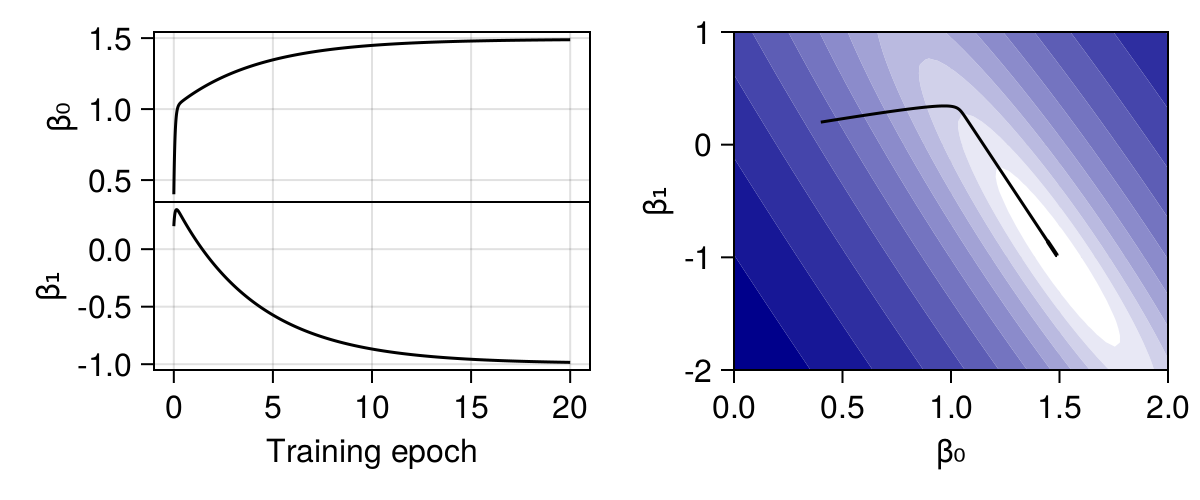
\includegraphics{chapters/gradientdescent_files/figure-pdf/fig-gradient-param-change-output-1.png}

}

\sidecaption{\label{fig-gradient-param-change}This figure shows the
change in the parameters values over time. Note that the change is very
large initially, because we make large steps when the gradient is
strong. The rate of change gets much lower as we get nearer to the
``correct'' value.}

\end{figure}%

This is what gives rise to the ``elbow'' shape in the right panel of
Figure~\ref{fig-gradient-param-change}. Remember that the gradient
descent algorithm, in its simple formulation, assumes that we can
\emph{never} climb back up, \emph{i.e.} we never accept a costly move.
The trajectory of the parameters therefore represents the path that
brings them to the lowest point they can reach \emph{without} having to
temporarily recommend a worse solution.

But how good is the solution we have reached?

\subsection{Outcome of the model}\label{outcome-of-the-model}

We could read the performance of the model using the data in
Figure~\ref{fig-gradient-loss-comparison}, but what we \emph{really}
care about is the model's ability to tell us something about the data we
initially gave it. This is presented in
Figure~\ref{fig-gradient-fitted}. As we can see, the model is doing a
rather good job at capturing the relationship between the number of
species and the number of interactions.

\begin{figure}[bt]

\centering{

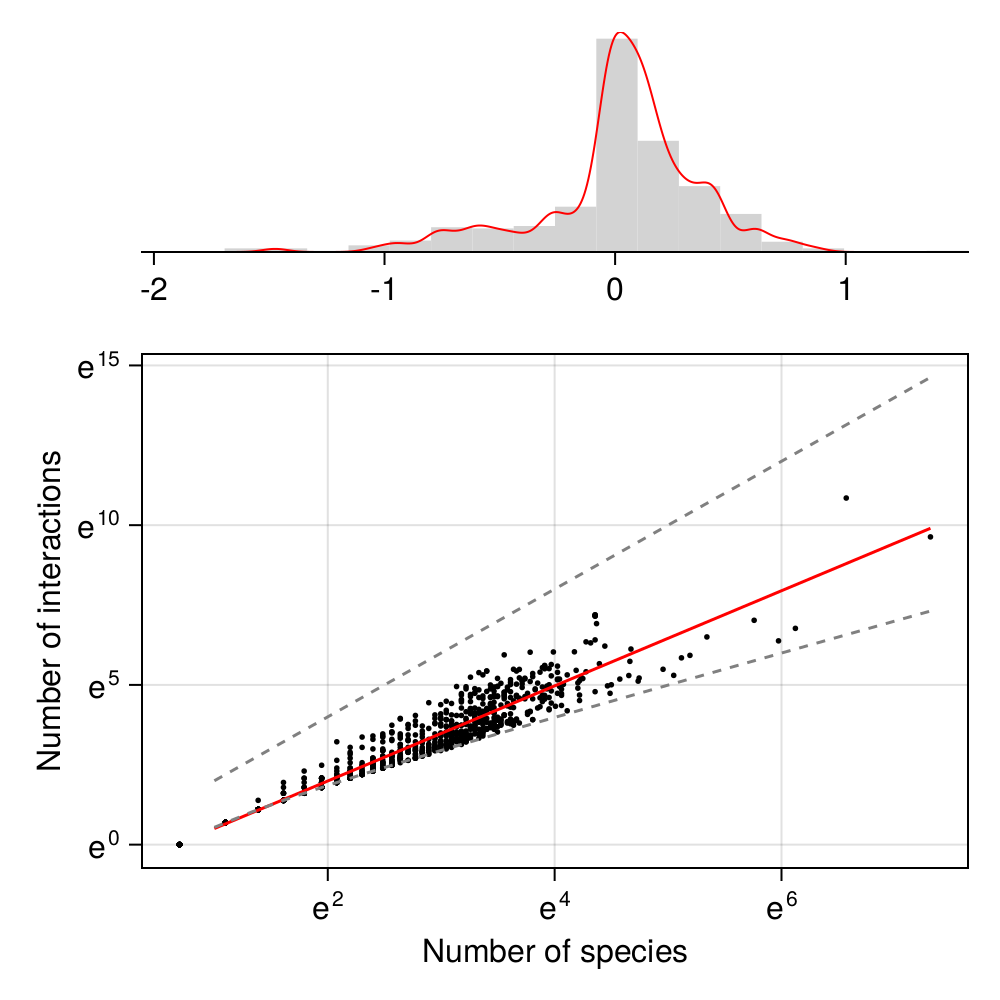
\includegraphics{chapters/gradientdescent_files/figure-pdf/fig-gradient-fitted-output-1.png}

}

\sidecaption{\label{fig-gradient-fitted}Overview of the fitted model.
The residuals (top panel) are mostly centered around 0, which suggests
little bias towards over/under predicting interactions. The red line
(based on the optimal coefficients) goes through the points, and
indicates a rather good fit of the model.}

\end{figure}%

We will have a far more nuanced discussion of ``what is this model good
for?'' in Chapter~\ref{sec-crossvalidation}, but for now, we can make a
decision about this model: it provides a good approximation of the
relationship between the species richness, and the number of
interactions, in a food web.

\section{A note on regularization}\label{a-note-on-regularization}

One delicate issue that we have avoided in this chapter is the absolute
value of the parameters. In other words, we didn't really care about how
large the model parameters would be, only the quality of the fit. This
is (generally) safe to do in a model with a single parameter. But what
if we had many different terms? What if, for example, we had a linear
model of the form \(\hat y \approx \beta_0 + \beta_1 x + \beta_2 x^2\)?
What if our model was of the form
\(\hat y \approx \beta_0 + \beta_1 x + \dots + \beta_n x^n\)? What if
\(n\) started to get very large compared to the number of data points?

In this situation, we would very likely see overfitting, wherein the
model would use the polynomial terms we provided to capture more and
more noise in the data. This would be a dangerous situation, as the
model will lose its ability to work on unknown data!

To prevent this situation, we may need to use regularization.
Thanfkully, regularization is a relatively simple process. In
Equation~\ref{eq-gradientdescent-gradientexplicit}, the function
\(f(p)\) we used to measure the gradient was the loss function directly.
In regularization, we use a slight variation on this, where

\[
f(p) = \text{loss} + \lambda \times g(\beta) \,,
\]

where \(\lambda\) is an hyper-parameter giving the strength of the
regularization, and \(g(\beta)\) is a function to calculate the total
penalty of a set of parameters.

When using \(L1\) regularization (LASSO regression),
\(g(\beta) = \sum |\beta|\), and when using \(L2\) regularization (ridge
regression), \(g(\beta) = \sum \beta^2\). When this gets larger, which
happens when the absolute value of the parameters increases, the model
is penalized. Note that if \(\lambda = 0\), we are back to the initial
formulation of the gradient, where the parameters have no direct effect
on the cost.

\section{Conclusion}\label{conclusion-1}

In this chapter, we have used a dataset of species richness and number
of interactions to start exploring the practice of machine learning. We
defined a model (a linear regression), and based about assumptions about
how to get closer to ideal parameters, we used the technique of gradient
descent to estimate the best possible relationship between \(S\) and
\(L\). In order to provide a fair evaluation of the performance of this
model, we kept a part of the dataset hidden from it while training. In
Chapter~\ref{sec-crossvalidation}, we will explore this last point in
great depth, by introducing the concept of cross-validation, testing
set, and performance evaluation.

\bookmarksetup{startatroot}

\chapter{Cross-validation}\label{sec-crossvalidation}

In Chapter~\ref{sec-clustering}, we were very lucky. Because we applied
an unsupervised method, we didn't really have a target to compare to the
output. Whatever classification we got, we had to live with it. It was
incredibly freeing. Sadly, in most applications, we will have to compare
our predictions to data, and data are incredibly vexatious. In this
chapter, we will develop intuitions on the notions of training, testing,
and validation.

In a sense, we started thinking about these concepts in
Chapter~\ref{sec-gradientdescent}; specifically, we came up with a way
to optimize the parameters of our model (\emph{i.e.} of \emph{training}
our model) based on a series of empirical observations, and a criteria
for what a ``good fit'' is. We further appraised the performance of our
model by measuring the loss (our measure of how good the fit is) on a
dataset that was not accessible during training, which we called the
\emph{testing} dataset. One issue with our approach in
Chapter~\ref{sec-gradientdescent} was that we had to set aside one out
of five observation for testing; in this chapter, we will explore more
advanced techniques to perform cross-validation.

\section{How can we split a dataset?}\label{how-can-we-split-a-dataset}

There is a much more important question to ask first: \emph{why} do we
split a dataset? In a sense, answering this question echoes the
discussion we started in Section~\ref{sec-gradientdescent-overfitting},
because the purpose of splitting a dataset is to ensure we can train and
evaluate it properly, in order to deliver the best possible model.

When a model is trained, it has learned from the data, we have tuned its
hyper-parameters to ensure that it learned with the best possible
conditions, and we have applied a measure of performance \emph{after}
the entire process is complete, to communicate how well we expect our
model to work. These three tasks require three different datasets, and
this is the purpose of splitting our data into groups.

One of the issues when reading about splitting data is that the
terminology can be muddy. For example, what constitutes a testing and
validation set can largely be a matter of perspective. In many
instances, testing and validation are used interchangeably, especially
when there is a single model involved. Nevertheless, it helps to settle
on a few guidelines here, before going into the details of what each
dataset constitutes and how to assemble it.

The \emph{training} instances are examples that are given to the model
during the training process. This dataset has the least ambiguous
definition. The training data is defined by subtraction, in a sense, as
whatever is left of the original data after we set aside testing and
validation sets.

The \emph{testing} instances are used at the end of the process, to
measure the performance of a trained model with tuned hyper-parameters.
If the training data are the lectures, testing data are the final exam:
we can measure the performance of the model on this dataset and report
it as the model performance we can expect when applying the model to new
data. There is a very important, chapter-long, caveat about this last
point, related to the potential of information leak between datasets,
which is covered in Chapter~\ref{sec-leakage}.

The \emph{validation} data are used in-between, as part of the training
process. They are (possibly) a subset of the training data that we use
internally to check the performance of the model, often in order to tune
its hyper-parameters, or as a way to report on the over-fitting of the
model during the training process.

The difference between testing and validation is largely a difference of
\emph{intent}. When we want to provide an \emph{a posteriori} assessment
of the model performance, the dataset we use to determine this
performance is a testing dataset. When we want to optimize some aspect
of the model, the data we use for this are the validation data. With
this high-level perspective in mind, let's look at each of these
datasets in turn. The differences between these three datasets are
summarized in Table~\ref{tbl-splits-models}.

\begin{longtable}[]{@{}
  >{\raggedright\arraybackslash}p{(\columnwidth - 6\tabcolsep) * \real{0.1600}}
  >{\raggedright\arraybackslash}p{(\columnwidth - 6\tabcolsep) * \real{0.1067}}
  >{\raggedright\arraybackslash}p{(\columnwidth - 6\tabcolsep) * \real{0.4400}}
  >{\raggedright\arraybackslash}p{(\columnwidth - 6\tabcolsep) * \real{0.2933}}@{}}
\caption{Overview of the three datasets used for training and
cross-validation. Information in the ``Data used for training'' column
refer to the data that have been used to train the model when
calculating its performance.}\label{tbl-splits-models}\tabularnewline
\toprule\noalign{}
\begin{minipage}[b]{\linewidth}\raggedright
Dataset
\end{minipage} & \begin{minipage}[b]{\linewidth}\raggedright
Trains
\end{minipage} & \begin{minipage}[b]{\linewidth}\raggedright
Purpose
\end{minipage} & \begin{minipage}[b]{\linewidth}\raggedright
Data used for training
\end{minipage} \\
\midrule\noalign{}
\endfirsthead
\toprule\noalign{}
\begin{minipage}[b]{\linewidth}\raggedright
Dataset
\end{minipage} & \begin{minipage}[b]{\linewidth}\raggedright
Trains
\end{minipage} & \begin{minipage}[b]{\linewidth}\raggedright
Purpose
\end{minipage} & \begin{minipage}[b]{\linewidth}\raggedright
Data used for training
\end{minipage} \\
\midrule\noalign{}
\endhead
\bottomrule\noalign{}
\endlastfoot
Training & yes & train model & \\
Validation & & validate during training & training data only \\
Testing & & estimates of future performance & all except testing \\
\end{longtable}

\subsection{Training}\label{training}

In data science (in applied machine learning in particular), we do not
\emph{fit} models. We \emph{train} them. This is an important
difference: training is an iterative process, that we can repeat,
optimize, and tweak. The outcome of training and the outcome of fitting
are essentially the same (a model that is parameterized to work as well
as possible on a given dataset), but it is good practice to adopt the
language of a field, and the language of data science emphasizes the
different practices in model training.

Training, to provide a general definition, is the action of modifying
the parameters of a model, based on knowledge of the data, and the error
that results from using the current parameter values. In
Chapter~\ref{sec-gradientdescent}, for example, we saw how to train a
linear model using the technique of gradient descent, based on a
specific dataset, with a learning rate and loss function we picked based
on trial and error. Our focus in this chapter is not on the methods we
use for training, but on the data that are required to train a model.

Training a model is a process akin to rote learning: we will present the
same input, and the same expected responses, many times over, and we
will find ways for the error on each response to decrease.

In order to initiate this process, we need an untrained model.
Untrained, in this context, refers to a model that has not been trained
\emph{on the specific problem} we are addressing; the model may have
been trained on a different problem (for example, we want to predict the
distribution of a species based on a GLM trained on a phylogenetically
related species). It is important to note that by ``training the
model'', what we really mean is ``change the structure of the parameters
until the output looks right''. For example, assuming a simple linear
model like \(c(X) = \beta_0 + \beta_1X_1 + \beta_2X_2\), training this
model would lead to changes in the values of \(\beta\), but not to the
consideration of a new model
\(c(X) = \beta_0 + \beta_1X_1 + \beta_2X_2 + \beta_3X_1X_2\). Comparing
models is (often) the point of validation, which we will address later
on.

\subsection{Validating}\label{validating}

The easiest way to think about the validation dataset is by thinking
about what it is \emph{not} used for: training the model (this is the
training set), and giving a final overview of the model expected
performance (this is the testing set). The validation set is used for
everything else (model selection, cross-validation, hyper-parameters
tuning), albeit in a specific way. With the training set, we communicate
the predictors and the labels to the model, and update the weights of
the model in response. With the validation set, we communicate the
predictors and the labels to the model, but we do \emph{not} update the
weights in response. All we care about during validation is the
performance of the model on a problem it has not yet encountered during
this specific round of training. If the training set is like attending a
lecture, the validation set is formative feedback.

Of course, one issue with the creation of a validation set is that it
needs to resemble the problem the model will have to solve in practice.
We will discuss this more in depth in the following sections, but it is
worth thinking about an example. Assume a model that classifies a
picture as having either a black bear, or no black bear. Now, we can
train this model using, for example, images from 10 camera traps that
are situated in a forest. And we might want to validate with a camera
trap that is in a zoo. In one of the enclosures. The one with a bear. A
polar one.

The issue with this dataset as a validation dataset is that is does not
matches the problem we try to solve in many different ways. First, we
will have an excess of images with bears compared to our problem
environment. Camera traps can have a large number of spurious
activation, resulting in images without animals in them (Newey \emph{et
al.} 2015). Second, the data will come from very different environments
(forest v. zoo). Finally, we are attempting to validate on something
that is an entirely different species of bear. This sounds like an
egregious case (it is), but it is easy to commit this type of mistake
when our data get more complex than black bear, polar bear, no bear.

Validation is, in particular, very difficult when the dataset we use for
training has extreme events (Bellocchi \emph{et al.} 2010). Similarly,
the efficiency of validation datasets can be limited if it reflects the
same biases as the training data (Martinez-Meyer 2005). Recall that this
validation dataset is used to decide on the ideal conditions to train
the final model before testing (and eventually, deployment); it is,
therefore, extremely important to get it right. A large number of
techniques to split data (Goot 2021; Søgaard \emph{et al.} 2021) use
heuristics to minimize the risk of picking the wrong validation data.

\subsection{Testing}\label{testing}

The testing dataset is special. The model has \emph{never} touched it.
Not during training, and not for validation. For this reason, we can
give it a very unique status: it is an analogue to data that are newly
collected, and ready to be passed through the trained model in order to
make a prediction.

The only difference between the testing set and actual new data is that,
for the testing set, we know the labels. In other words, we can compare
the model output to these labels, and this gives us an estimate of the
model performance on future data. Assuming that this data selection was
representative of the real data we will use for our model once it is
trained, the performance on the validation set should be a good baseline
for what to expect in production.

But this requires a trained model, and we sort of glossed over this
step.

In order to come up with a trained model, it would be a strange idea not
to use the validation data -- they are, after all, holding information
about the data we want to model! Once we have evaluated our model on the
validation set, we can start the last round of training to produce the
final model. We do this by training the model using everything
\emph{except} the testing data. This is an appropriate thing to do:
because we have evaluated the model on the validation data, and assuming
that it has a correct performance, we can expect that retraining the
model on the validation data will not change the performance of the
model.

\section{The problem: cherry blossom
phenology}\label{the-problem-cherry-blossom-phenology}

The cherry blossom tree (\emph{Prunus}) is renowned for its impressive
bloom, which happens from March to April. The blooming, and associated
festivals, are of particular cultural significance (Moriuchi \& Basil
2019), and is therefore a cultural ecosystem service (Kosanic \& Petzold
2020). Climate change has a demonstrable effect on the date of first
bloom on \emph{Prunus} species in Japan (Primack \emph{et al.} 2009),
which can affect the sustainability of cherry blossom festivals in the
short term (Sakurai \emph{et al.} 2011).

Long-term time series of the date of first bloom in Japan reveal that in
the last decades, cherry blossom blooms earlier, which has been linked
to, possibly, climate change and urbanization. \emph{Prunus} species
respond to environmental cues at the local level for their flowering
(Mimet \emph{et al.} 2009; Ohashi \emph{et al.} 2011). The suspected
causal mechanism is as follows: both global warming and urbanization
lead to higher temperatures, which means a faster accumulation of degree
days over the growing season, leading to an earlier bloom (Shi \emph{et
al.} 2017). Indeed, the raw data presented in
Figure~\ref{fig-splits-rawdata} show that trees bloom early when the
temperatures are higher; the data for phenology have been collected by
Aono \& Kazui (2008), and the temperature reconstructions are from Aono
\& Saito (2009).

\begin{figure}[bt]

\centering{

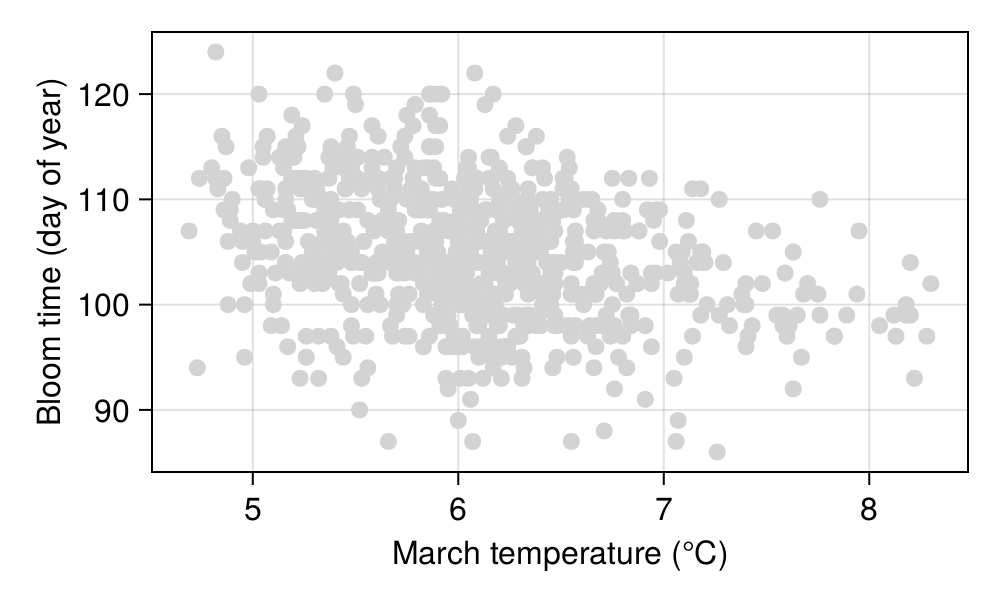
\includegraphics{chapters/crossvalidation_files/figure-pdf/fig-splits-rawdata-output-1.png}

}

\sidecaption{\label{fig-splits-rawdata}The raw data show a negative
relationship between the temperature in March, and the bloom time. This
suggests that when the trees have accumulated enough temperature, they
can bloom early. In a context of warming, we should therefore see
earlier blooms with rising temperatures.}

\end{figure}%

With these data in hand (day of year with the first bloom, and smoothed
reconstructed temperature in March), we can start thinking about this
hypothesis. But by contrast with our simple strategy in
Chapter~\ref{sec-gradientdescent}, this time, we will split our dataset
into training, validation, and testing sets, as we discussed in the
previous section. Yet there are many ways to split a dataset, and
therefore before starting the analysis, we will have a look at a few of
them.

\section{Strategies to split data}\label{strategies-to-split-data}

Before seeing examples of strategies for cross-validation, it is
important to consider the high-level perspective of the way we will
perform the entire training sequence. First, we need to keep a testing
dataset. Depending on the problem, it may be \emph{feasible} or
\emph{desirable} to use an external testing dataset (Homeyer \emph{et
al.} 2022). In problems for which the volume of data is limited (the
99.99\% of biodiversity applications that do not involve metagenomics of
remote sensing), this is almost impossible, and therefore we need to
resort to removing a proportion of the data. It means that collected
data will never be used for training, which is not ideal, but what we
gain in return is a fairer appraisal of the performance of the model,
which is a really advantageous trade-off. When the testing data are
removed, we can start splitting the rest of the data in testing and
validation sets. This can involve two broad categories of families:
exhaustive splits (all data are used for training and evaluation), and
non-exhaustive splits (the opposite; for once, the terminology makes
sense!).

\subsection{Holdout}\label{holdout}

The holdout method is what we used in Chapter~\ref{sec-gradientdescent},
in which we randomly selected some observations to be part of the
validation data (which was, in practice, a testing dataset in this
example), and kept the rest to serve as the training data. Holdout
cross-validation is possibly the simplest technique, but it suffers from
a few drawbacks.

The model is only trained for one split of the data, and similarly only
evaluated for one split of the data. There is, therefore, a chance to
sample a particularly bad combination of the data that lead to erroneous
results. Attempts to quantify the importance of the predictors are
likely to give particularly unstable results, as the noise introduced by
picking a single random subset will not be smoothed out by multiple
attempts.

In addition, as Hawkins \emph{et al.} (2003) point out, holdout
validation is particularly wasteful in data-limited settings, where
there are fewer than hundreds of observations. The reason is that the
holdout dataset will \emph{never} contribute to training, and assuming
the data are split 80/20, one out of five observations will not
contribute to the model. Other cross-validation schemes presented in
this section will allow observations to be used both for training and
validation.

\subsection{Leave-p-out}\label{leave-p-out}

In leave-\emph{p}-out cross-validation (LpOCV), starting from a dataset
on \(n\) observations, we pick \(p\) at random to serve as validation
data, and \(n-p\) to serve as the training dataset. This process is then
repeated \emph{exhaustively}, which is to say we split the dataset in
every possible way that gives \(p\) and \(n-p\) observations, for a set
value of \(p\). The model is then trained on the \(n-p\) observations,
and validated on the \(p\) observations for validation, and the
performance (or loss) is averaged to give the model performance before
testing.

Celisse (2014) points out that \(p\) has to be large enough (relative to
the sample size \(n\)) to overcome the propensity of the model to
overfit on a small training dataset. One issue with LpOCV is that the
number of combinations is potentially very large. It is, in fact, given
by the binomial coefficient \(\binom{n}{p}\), which gets unreasonably
large even for small datasets. For example, running LpOCV on \(n=150\)
observations, leaving out \(p=10\) for validation every time, would
require to train the model about \(10^{15}\) times. Assuming we can
train the model in \(10^{-3}\) seconds, the entire process would require
370 centuries.

Oh well.

\subsection{Leave-one-out}\label{leave-one-out}

The leave-one-out cross-validation (LOOCV) is a special case of LpOCV
with \(p=1\). Note that it is a lot faster to run than LpOCV, because
\(\binom{n}{1}=n\), and so the validation step runs in
\(\mathcal{O}(n)\) (LpOCV runs in \(\mathcal{O}(n!)\)). LOOCV is also an
\emph{exhaustive} cross-validation technique, as every possible way to
split the dataset will be used for training and evaluation.

\subsection{k-fold}\label{k-fold}

One of the most frequent cross-validation scheme is k-fold
cross-validation. Under this approach, the dataset is split into \(k\)
equal parts (and so when \(k = n\), this is also equivalent to LOOCV).
Like with LOOCV, one desirable property of k-fold cross-validation is
that each observation is used \emph{exactly} one time to evaluate the
model , and \emph{exactly} \(k-1\) times to train it.

But by contrast with the holdout validation approach, \emph{all}
observations are used to train the model.

When the data have some specific structure, it can be a good thing to
manipulate the splits in order to maintain this structure. For example,
Bergmeir \& Benítez (2012) use temporal blocks for validation of time
series, and retain the last part of the series for testing (we
illustrate this in Figure~\ref{fig-splits-illustration}). For spatial
data, Hijmans (2012) suggests the use of a null model based on distance
to training sites to decide on how to split the data; Valavi \emph{et
al.} (2018) have designed specific k-fold cross-validation schemes for
species distribution models. These approaches all belong to the family
of \emph{stratified} k-fold cross-validation (Zeng \& Martinez 2000).

\begin{figure}[bt]

\centering{

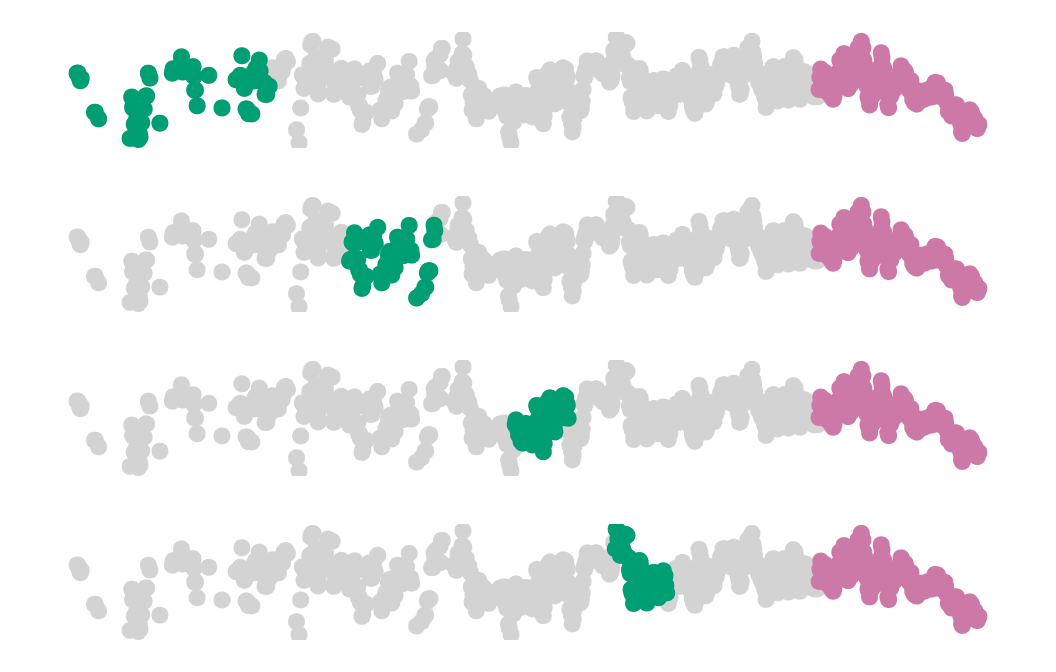
\includegraphics{chapters/crossvalidation_files/figure-pdf/fig-splits-illustration-output-1.png}

}

\sidecaption{\label{fig-splits-illustration}An illustration of a series
of folds on a timeseries. The grey data are used for training, the green
data for validation, and the purple data are kept for testing. Note that
in this context, we sometimes use the future to validate on the past
(look at the first fold!), but this is acceptable for reasons explained
in the text.}

\end{figure}%

The appropriate value of \(k\) is often an unknown. It is common to use
\(k = 10\) as a starting point (tenfold cross-validation), but other
values are justifiable based on data volume, or complexity of the model
training, to name a few.

\subsection{Monte-Carlo}\label{monte-carlo}

One limitation of k-fold cross-validation is that the number of splits
is limited by the amount of observations, especially if we want to
ensure that there are enough samples in the validation data. To
compensate for this, Monte-Carlo cross-validation is essentially the
application (and averaging) of holdout validation an arbitrary number of
times. Furthermore, the training and validation datasets can be
constructed in order to account for specific constraints in the dataset,
giving more flexibility than k-fold cross-validation. When the
(computational) cost of training the model is high, and the dataset has
specific structural constraints, Monte-Carlo cross-validation is a good
way to generate data for hyperparameters tuning.

One issue with Monte-Carlo cross-validation is that we lose the
guarantee that every observation will be used for training at least once
(and similarly for validation). Trivially, this becomes less of an issue
when we increase the number of replications, but then this suffers from
the same issues as LpOCV, namely the unreasonable computational
requirements.

\section{Application: when do cherry blossom
bloom?}\label{application-when-do-cherry-blossom-bloom}

The model we will train for this section is really simple:
\(\text{bloom day} = m \times \text{temperature} + b\). This is a linear
model, and one with a nice, direct biological interpretation: the
average (baseline) day of bloom is \(b\), and each degree of temperature
expected in March adds \(m\) days to the bloom date. At this point, we
\emph{might} start thinking about the distribution of the response, and
what type of GLM we should used, but no. Not today. Today, we want to
iterate quickly, and so we will start with a model that is exactly as
simple as it needs to be: this is, in our case, linear regression.

At this point, we may be tempted to think a little more deeply about the
variables and the structure of the model, to express the bloom day as a
departure from the expected value, and similarly with the temperature,
using for example the \emph{z}-score. This is a transformation we will
apply starting from Chapter~\ref{sec-classification}, but in order to
apply it properly, we need to consider some elements that will be
introduced in Chapter~\ref{sec-leakage}. For this reason, we will not
apply any transformation to the data yet; feel free to revisit this
exercise after reading through Chapter~\ref{sec-leakage}.

This approach (start from a model that is suspiciously simple) is a good
thing, for more than a few reasons. First, it gives us a baseline to
compare more complicated models against. Second, it means that we do not
need to focus on the complexity of the code (and the model) when
building a pipeline for the analysis. Finally, and most importantly, it
gives us a result very rapidly, which enables a loop of iterative model
refinement on a very short timescale. Additionally, at least for this
example, the simple models often work well enough to support a
discussion of the model and training process.

\subsection{Performance evaluation}\label{performance-evaluation}

We can visualize the results of our model training and assessment
process. These results are presented in
Figure~\ref{fig-splits-performance} (as well as in
Table~\ref{tbl-splits-performance-summary}, if you want to see the
standard deviation across all splits), and follow the same color-coding
convention we have used so far. All three loss measures presented here
express their loss in the units of the response variable, which in this
case is the day of the year where the bloom was recorded. These results
show that our trained model achieves a loss of the order of a day or two
in the testing data, which sounds really good!

\begin{figure}[bt]

\centering{

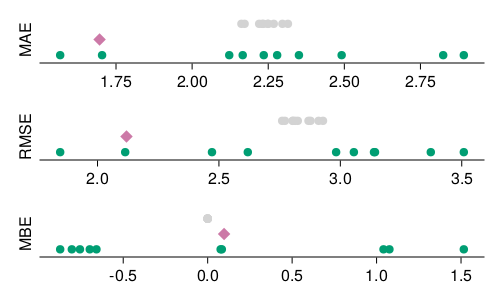
\includegraphics{chapters/crossvalidation_files/figure-pdf/fig-splits-performance-output-1.png}

}

\sidecaption{\label{fig-splits-performance}Visualisation of the model
performance for three loss functions (MA, RMSE, MBE, as defined in
Table~\ref{tbl-gradientdescent-regressionloss}). The colors are the same
as in Figure~\ref{fig-splits-illustration}, \emph{i.e.} grey for the
training data, green for the validation data, and purple for the testing
data.}

\end{figure}%

Yet it is important to contextualize these results. What does it means
for our prediction to be correct plus or minus two days? There are at
least two important points to consider.

\begin{table}

\caption{\label{tbl-splits-performance-summary}TODO}

\centering{

\begin{longtable}[]{@{}rrrr@{}}
\toprule\noalign{}
Dataset & Measure & Loss (avg.) & Loss (std. dev.) \\
\midrule\noalign{}
\endhead
\bottomrule\noalign{}
\endlastfoot
Testing & MAE & 1.696 & \\
Training & MAE & 2.2397 & 0.0482364 \\
Validation & MAE & 2.26331 & 0.421513 \\
Testing & MBE & 0.0971036 & \\
Training & MBE & 9.8278e-15 & 1.15597e-14 \\
Validation & MBE & 0.000419595 & 0.910229 \\
Testing & MSE & 4.49123 & \\
Training & MSE & 8.04855 & 0.32487 \\
Validation & MSE & 8.24897 & 2.93094 \\
Testing & RMSE & 2.11925 & \\
Training & RMSE & 2.83648 & 0.0570941 \\
Validation & RMSE & 2.82514 & 0.545232 \\
\end{longtable}

}

\end{table}%

First, what are we predicting? Our response variable is not
\emph{really} the day of the bloom, but is rather a smoothed average
looking back some years, and looking ahead some years too. For this
reason, we are removing a lot of the variability in the underlying time
series. This is not necessarily a bad thing, especially if we are
looking for a trend at a large temporal scale, but it means that we
should not interpret our results at a scale lower than the duration of
the window we use for averaging.

Second, what difference \emph{does} a day make?
Figure~\ref{fig-splits-rawdata} shows that most of the days of bloom
happen between day-of-year 100 and day-of-year 110. Recall that the MAE
is measured by taking the average absolute error -- a mistake of 24
hours is 10\% of this interval! This is an example of how thinking about
the units of the loss function we use for model evaluation can help us
contextualize the predictions, and in particular how actionable they can
be.

\subsection{Model predictions}\label{model-predictions}

The predictions of our model are presented in
Figure~\ref{fig-splits-prediction}; these are the predictions of the
\emph{final} model, that is, the model that we trained on everything
\emph{except} the testing data, and for which we can get the performance
by looking at Figure~\ref{fig-splits-performance}.

\begin{figure}[bt]

\centering{

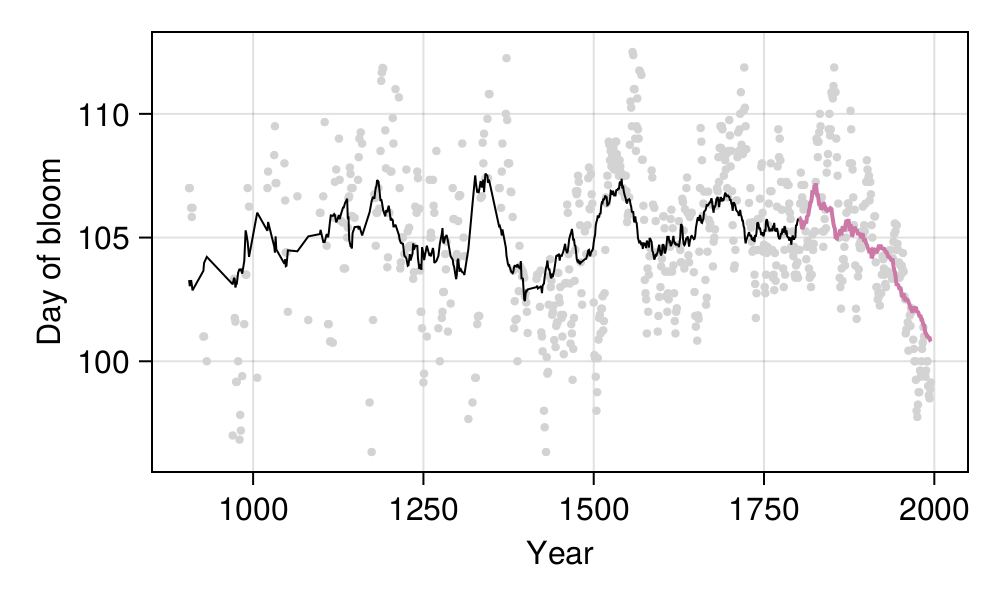
\includegraphics{chapters/crossvalidation_files/figure-pdf/fig-splits-prediction-output-1.png}

}

\sidecaption{\label{fig-splits-prediction}TODO}

\end{figure}%

The question we now need to answer is: is our model doing a good job? We
can start thinking about this question in a very qualitative way: yes,
it does a goob job at drawing a line that, through time, goes right
through the original data more often that it doesn't. As far as
validation goes, it maybe underestimates the drop in the response
variable (it predicts the bloom a little later), but maybe there are
long-term effects, expressed over the lifetime of the tree (the first
bloom usually takes places after 6 or 7 growth seasons), that we do not
account for.

\marginnote{\begin{footnotesize}

Think about the structure of linear models. Can we use information about
the previous years in our model? Would there be a risk associated to
adding more parameters?

\end{footnotesize}}

Our model tends to smooth out some of the variation; it does not predict
bloom dates before day of year 100, or after day of year 108, although
they do happen. This may not be a trivial under-prediction: some of
these cycles leading to very early/late bloom can take place over a
century, meaning that our model could be consistently wrong (which is to
say, wrong with the same bias) for dozens of years in a row.

\subsection{Is our model good, then?}\label{sec-crossvalidation-fitness}

The answer is, it depends. Models are neither good, nor bad. They are
either fit, or unfit, for a specific purpose.

If the purpose is to decide when to schedule a one-day trip to see the
cherry blossom bloom, our model is not really fit -- looking at the
predictions, it gets within a day of the date of bloom (but oh, by the
way, this is an average over almost a decade!) about 15\% of the time,
which jumps up to almost 30\% if you accept a two-days window of error.

If the purpose is to look at long-time trends in the date of bloom, then
our model actually works rather well. It does under-estimate the
amplitude of the cycles, but not by a large amount. In fact, we could
probably stretch the predictions a little, applying a little correction
factor, and have a far more interesting model.

We will often be confronted to this question when working with
prediction. There is not really a criteria for ``good'', only a series
of compromises and judgment calls about ``good enough''. This is
important. It reinforces the imperative of keeping the practice of data
science connected to the domain knowledge, as ultimately, a domain
expert will have to settle on whether to use a model or not.

\begin{figure}[bt]

\centering{

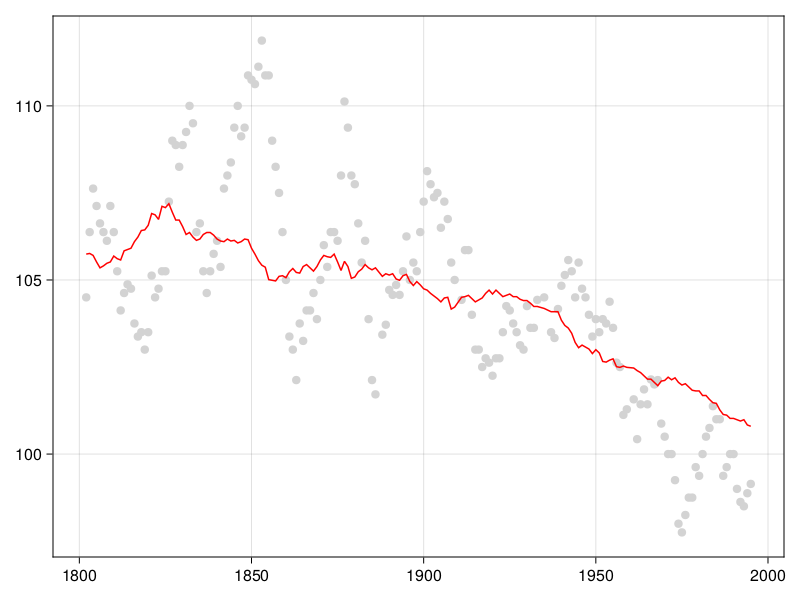
\includegraphics{chapters/crossvalidation_files/figure-pdf/fig-splits-detail-output-1.png}

}

\sidecaption{\label{fig-splits-detail}TODO}

\end{figure}%

\bookmarksetup{startatroot}

\chapter{Data leakage}\label{sec-leakage}

Data leakage is a concept that is, surprisingly, grosser than it sounds.
The purpose of this section is to put the fear of data leakage in you,
because it can, and most assuredly \emph{will}, lead to bad models,
which is to say (as we discussed in
Section~\ref{sec-gradientdescent-trainedmodel}), models that do not
adequately represent the underlying data, in part because we have
built-in some biases into them. In turn, this can eventually lead to
decreased explainability of the models, which erodes trust in their
predictions (Amarasinghe \emph{et al.} 2023). As illustrated by Stock
\emph{et al.} (2023), a large number of ecological applications of
machine learning are particularly susceptible to data leakage, meaning
that this should be a core point of concern for us.

\section{Consequences of data leakage}\label{sec-leakage-consequences}

We take data leakage so seriously because it is one of the top ten
mistakes in applied machine learning (Nisbet \emph{et al.} 2018). Data
leakage happens information ``leaks'' from the training conditions to
the evaluation conditions. In other words, when the model is evaluated
after mistakenly being fed information that would not be available in
real-life situations. Note that this definition of leakage is different
from another notion, namely the loss of data availability over time
(Peterson \emph{et al.} 2018).

It is worth stopping for a moment to consider what these ``real-life
situations'' are, and how they differ from the training of the model.
Most of this difference can be summarized by the fact that when we are
\emph{applying} a model, we can start from the model \emph{only}. Which
is to say, the data that have been used for the training and validation
of the model may have been lost, without changing the applicability of
the model: it works on entirely new data.

Because this is the behavior we want to simulate with a validation
dataset, it is very important to fully disconnect the validation data
from the rest of the data. We can illustrate this with an example. Let's
say we want to work on a time series of population size, such as
provided by the \emph{BioTIME} project (Dornelas \emph{et al.} 2018).
One naïve approach would be to split this the time series at random into
three datasets. We can use one to train the models, one to test these
models, and a last one for validation.

Congratulations! We have created data leakage! Because we are splitting
our timeseries at random, the model will likely have been trained using
data that date from \emph{after} the start of the validation dataset. In
other words: our model can peek into the future. This is highly unlikely
to happen in practice, due to the laws of physics. A strategy that would
prevent leakage would have been to pick a cut-off date to define the
validation dataset, and then to decide how to deal with the training and
testing sets.

\textbf{TODO} stationary processes Politis \& Romano (1994)

\section{Sources of data leakage}\label{leakage-sec-leakage-sources}

\subsection{Leakage between instances}\label{leakage-between-instances}

\subsection{Leakage between features}\label{leakage-between-features}

\subsection{Leakage during
transformations}\label{leakage-during-transformations}

\section{Avoiding data leakage}\label{leakage-sec-leakage-avoid}

The most common advice given in order to prevent data leakage is the
``learn/predict separation'' (Kaufman \emph{et al.} 2011). Simply put,
this means that whatever happens to the data used for training cannot be
\emph{simultaneously} applied to the data used for testing (or
validation).

\subsection{An example using PCA}\label{an-example-using-pca}

Assume that we want to transform our data using a Principal Component
Analysis (PCA; Pearson (1901)). Ecologists often think of PCA as a
technique to explore data (Legendre \& Legendre 2012), but it is so much
more than that! PCA is a model, because we can derive, from the data, a
series of weights (in the transformation matrix), which we can then
apply to other datasets in order to project them in the space of the
projection of the training data.

If we have a dataset \(\mathbf{X}\), which we split into two components
\(\mathbf{X}_0\) for training ,and \(\mathbf{X}_1\) for validation,
there are two ways to use a PCA to transform these data. The first is
\(\mathbf{T} = \mathbf{X}\mathbf{W}\), which uses the full dataset. When
we predict the position of the validation data, we could use the
transformation \(\mathbf{T}_1 = \mathbf{X}_1\mathbf{W}\), but this would
introduce data leakage: we have trained the transformation we apply to
\(\mathbf{X}_1\) using data that are already in \(\mathbf{X}_1\), and
therefore we have not respected the learn/predict separation.

The second way to handle this situation is to perform our PCA using
\(\mathbf{T}_0 = \mathbf{X}_0\mathbf{W}_0\), which is to say, the
weights of our PCA are derived \emph{only} from the training data. In
this situation, whenever we project the data in the validation set using
\(\mathbf{T}_1 = \mathbf{X}_1\mathbf{W}_0\), we respect the
learn/predict separation: the transformation of \(\mathbf{X}_1\) is
entirely independent from the data contained in \(\mathbf{X}_1\).

\subsection{How to generalize this
approach?}\label{how-to-generalize-this-approach}

Although avoiding data leakage is a tricky problem, there is a very
specific mindset we can adopt that goes a long way towards not
introducing it in our analyses, and it is as follows: \emph{every data
transformation step is a modeling step that is part of the learning
process}.

Everything is a model that can be trained. If you want to transform a
variable using the z-score, this is a model! It has two parameters that
you can learn from the data, \(\mu\) (the average of the variable) and
\(\sigma\) (its standard deviation). You can apply it to a data point
\(y\) with \(\hat y = (y - \mu)\sigma^{-1}\) Because this is a model, we
need a dataset to learn these parameters from, and because we want to
maintain the learn/predict separation, we will use the train dataset to
get the values of \(\mu_0\) and \(\sigma_0\). This way, when we want to
get the z-score of a new observation, for example from the testing
dataset, we can get it using \(\hat y_1 = (y_1 - \mu_0)\sigma_0^{-1}\).
The data transformation is entirely coming from information that was
part of the training set.

One way to get the learn/predict transformation stupendously wrong is to
transform our validation, testing, or prediction data using
\(\hat y_1 = (y_1 - \mu_1)\sigma_1^{-1}\). This can be easily understood
with an example. Assume that the variable \(y_0\) is the temperature in
our training dataset. We are interested in making a prediction in a
world that is 2 degrees hotter, uniformly, which is to say that for
whatever value of \(y_0\), the corresponding data point we use for
prediction is \(y_1 = y_0 + 2\). If we take the z-score of this new
value based on its own average and standard deviation, a temperature two
degrees warmer in the prediction data will have the same z-score as its
original value, or in other words, we have hidden the fact that there is
a change in our predictors! Although this would not make a difference if
we are reasonably confident that our predictors are stationary
processes, there is no good reason to make this assumption.

Treating the data preparation step as a part of the learning process,
which is to say that we learn every transformation on the training set,
and retain this transformation as part of the prediction process, we are
protecting ourselves against both data leakage and the hiding of
relevant changes in our predictors.

\bookmarksetup{startatroot}

\chapter{Supervised classification}\label{sec-classification}

In the previous chapters, we have focused on efforts on regression
models, which is to say models that predict a continuous response. In
this chapter, we will introduce the notion of classification, which is
the prediction of a discrete variable representing a category. There are
a lot of topics we need to cover before we can confidently come up with
a model for classification, and so this chapter is part of a series. We
will first introduce the idea of classification; in
Chapter~\ref{sec-variable-selection}, we will explore techniques to
fine-tune the set of variables we use for prediction; in
Chapter~\ref{sec-tuning}, we will think about predictions of classes as
probabilities, and generalize these ideas and think about learning
curves; finally, in Chapter~\ref{sec-explanations}, we will think about
variables a lot more, and introduce elements of model interpretability.

\bookmarksetup{startatroot}

\chapter{Variable selection}\label{sec-variable-selection}

\bookmarksetup{startatroot}

\chapter{Learning curves and moving thresholds}\label{sec-tuning}

In Chapter~\ref{sec-gradientdescent}, we represented the testing and
training loss of a model as a function of the number of gradient descent
steps we had made. This sort of representation is very useful to figure
out how well our model is learning, and is called, appropriately enough,
a learning curve. In this chapter, we will produce learning curves to
find the optimal values of hyper-parameters of our model. We will
illustrate this using an approach called moving-threshold
classification, and additionally explore how we can conduct grid
searches to tune several hyper-parameters at once.

\bookmarksetup{startatroot}

\chapter{Explaining predictions}\label{sec-explanations}

In this chapter, we will

navigate the accuracy-explainability for public policy Bell \emph{et
al.} (2022)

what is explainable differs between stakeholders Amarasinghe \emph{et
al.} (2023)

biodiversity need sustained model uptake Weiskopf \emph{et al.} (2022)

Štrumbelj \& Kononenko (2013) monte carlo approximation of shapley
values

Wadoux \emph{et al.} (2023) mapping of shapley values

Mesgaran \emph{et al.} (2014) mapping of most important covariates

Lundberg \& Lee (2017) SHAP

\bookmarksetup{startatroot}

\chapter*{References}\label{references}
\addcontentsline{toc}{chapter}{References}

\markboth{References}{References}

\phantomsection\label{refs}
\begin{CSLReferences}{1}{0}
\bibitem[\citeproctext]{ref-aloise2009}
Aloise, D., Deshpande, A., Hansen, P. \& Popat, P. (2009).
\href{https://doi.org/10.1007/s10994-009-5103-0}{NP-hardness of
Euclidean sum-of-squares clustering}. \emph{Machine Learning}, 75,
245--248.

\bibitem[\citeproctext]{ref-amarasinghe2023}
Amarasinghe, K., Rodolfa, K.T., Lamba, H. \& Ghani, R. (2023).
\href{https://doi.org/10.1017/dap.2023.2}{Explainable machine learning
for public policy: Use cases, gaps, and research directions}. \emph{Data
\& Policy}, 5.

\bibitem[\citeproctext]{ref-anderson1928}
Anderson, E. (1928). \href{https://doi.org/10.2307/2394087}{The problem
of species in the northern blue flags, iris versicolor l. And iris
virginica l.} \emph{Annals of the Missouri Botanical Garden}, 15, 241.

\bibitem[\citeproctext]{ref-aono2008}
Aono, Y. \& Kazui, K. (2008).
\href{https://doi.org/10.1002/joc.1594}{Phenological data series of
cherry tree flowering in Kyoto, Japan, and its application to
reconstruction of springtime temperatures since the 9th century}.
\emph{International Journal of Climatology}, 28, 905--914.

\bibitem[\citeproctext]{ref-aono2009}
Aono, Y. \& Saito, S. (2009).
\href{https://doi.org/10.1007/s00484-009-0272-x}{Clarifying springtime
temperature reconstructions of the medieval period by gap-filling the
cherry blossom phenological data series at Kyoto, Japan}.
\emph{International Journal of Biometeorology}, 54, 211--219.

\bibitem[\citeproctext]{ref-bell2022}
Bell, A., Solano-Kamaiko, I., Nov, O. \& Stoyanovich, J. (2022).
\href{https://doi.org/10.1145/3531146.3533090}{It{'}s just not that
simple: An empirical study of the accuracy-explainability trade-off in
machine learning for public policy}. \emph{2022 ACM Conference on
Fairness, Accountability, and Transparency}.

\bibitem[\citeproctext]{ref-bellocchi2010}
Bellocchi, G., Rivington, M., Donatelli, M. \& Matthews, K. (2010).
\href{https://doi.org/10.1051/agro/2009001}{Validation of biophysical
models: issues and methodologies. A review}. \emph{Agronomy for
Sustainable Development}, 30, 109--130.

\bibitem[\citeproctext]{ref-bergmeir2012}
Bergmeir, C. \& Benítez, J.M. (2012).
\href{https://doi.org/10.1016/j.ins.2011.12.028}{On the use of
cross-validation for time series predictor evaluation}.
\emph{Information Sciences}, 191, 192--213.

\bibitem[\citeproctext]{ref-bezanson2017}
Bezanson, J., Edelman, A., Karpinski, S. \& Shah, V.B. (2017).
\href{https://doi.org/10.1137/141000671}{Julia: A Fresh Approach to
Numerical Computing}. \emph{SIAM Review}, 59, 65--98.

\bibitem[\citeproctext]{ref-blaom2020}
Blaom, A., Kiraly, F., Lienart, T., Simillides, Y., Arenas, D. \&
Vollmer, S. (2020). \href{https://doi.org/10.21105/joss.02704}{MLJ: A
julia package for composable machine learning}. \emph{Journal of Open
Source Software}, 5, 2704.

\bibitem[\citeproctext]{ref-bodmer2021}
Bodmer, W., Bailey, R.A., Charlesworth, B., Eyre-Walker, A., Farewell,
V., Mead, A., \emph{et al.} (2021).
\href{https://doi.org/10.1038/s41437-020-00394-6}{The outstanding
scientist, R.A. Fisher: his views on eugenics and race}.
\emph{Heredity}, 126, 565--576.

\bibitem[\citeproctext]{ref-brose2004}
Brose, U., Ostling, A., Harrison, K. \& Martinez, N.D. (2004).
\href{https://doi.org/10.1038/nature02297}{Unified spatial scaling of
species and their trophic interactions}. \emph{Nature}, 428, 167--171.

\bibitem[\citeproctext]{ref-celisse2014}
Celisse, A. (2014). \href{https://doi.org/10.1214/14-aos1240}{Optimal
cross-validation in density estimation with the
{\$}l{\^{}}{\textbraceleft}2{\textbraceright}{\$}-loss}. \emph{The
Annals of Statistics}, 42.

\bibitem[\citeproctext]{ref-cohen1984}
Cohen, J.E. \& Briand, F. (1984). Trophic links of community food webs.
\emph{Proc Natl Acad Sci U S A}, 81, 4105--4109.

\bibitem[\citeproctext]{ref-cooney2022}
Cooney, C.R., He, Y., Varley, Z.K., Nouri, L.O., Moody, C.J.A., Jardine,
M.D., \emph{et al.} (2022).
\href{https://doi.org/10.1038/s41559-022-01714-1}{Latitudinal gradients
in avian colourfulness}. \emph{Nature Ecology \& Evolution}, 6,
622--629.

\bibitem[\citeproctext]{ref-cooper2019}
Cooper, N., Bond, A.L., Davis, J.L., Portela Miguez, R., Tomsett, L. \&
Helgen, K.M. (2019). \href{https://doi.org/10.1098/rspb.2019.2025}{Sex
biases in bird and mammal natural history collections}.
\emph{Proceedings of the Royal Society B: Biological Sciences}, 286,
20192025.

\bibitem[\citeproctext]{ref-davies1979}
Davies, D.L. \& Bouldin, D.W. (1979).
\href{https://doi.org/10.1109/tpami.1979.4766909}{A cluster separation
measure}. \emph{IEEE Transactions on Pattern Analysis and Machine
Intelligence}, PAMI-1, 224--227.

\bibitem[\citeproctext]{ref-deisenroth2020}
Deisenroth, M.P., Faisal, A.A. \& Ong, C.S. (2020).
\href{https://doi.org/10.1017/9781108679930}{Mathematics for machine
learning}.

\bibitem[\citeproctext]{ref-dornelas2018}
Dornelas, M., Antão, L.H., Moyes, F., Bates, A.E., Magurran, A.E., Adam,
D., \emph{et al.} (2018).
\href{https://doi.org/10.1111/geb.12729}{BioTIME: A database of
biodiversity time series for the Anthropocene}. \emph{Global Ecology and
Biogeography}, 27, 760--786.

\bibitem[\citeproctext]{ref-dunn1974}
Dunn, J.C. (1974).
\href{https://doi.org/10.1080/01969727408546059}{Well-Separated Clusters
and Optimal Fuzzy Partitions}. \emph{Journal of Cybernetics}, 4,
95--104.

\bibitem[\citeproctext]{ref-fisher1936}
Fisher, R.A. (1936).
\href{https://doi.org/10.1111/j.1469-1809.1936.tb02137.x}{The Use Of
Multiple Measurements In Taxonomic Problems}. \emph{Annals of Eugenics},
7, 179--188.

\bibitem[\citeproctext]{ref-gonzalez2023}
Gonzalez, A., Vihervaara, P., Balvanera, P., Bates, A.E., Bayraktarov,
E., Bellingham, P.J., \emph{et al.} (2023).
\href{https://doi.org/10.1038/s41559-023-02171-0}{A global biodiversity
observing system to unite monitoring and guide action}. \emph{Nature
Ecology \& Evolution}.

\bibitem[\citeproctext]{ref-vandergoot2021}
Goot, R. van der. (2021).
\href{https://doi.org/10.18653/v1/2021.emnlp-main.368}{We need to talk
about train-dev-test splits}. \emph{Proceedings of the 2021 Conference
on Empirical Methods in Natural Language Processing}.

\bibitem[\citeproctext]{ref-gorman2014}
Gorman, K.B., Williams, T.D. \& Fraser, W.R. (2014).
\href{https://doi.org/10.1371/journal.pone.0090081}{Ecological Sexual
Dimorphism and Environmental Variability within a Community of Antarctic
Penguins (Genus Pygoscelis)}. \emph{PLoS ONE}, 9, e90081.

\bibitem[\citeproctext]{ref-gray1984}
Gray, R. (1984).
\href{https://doi.org/10.1109/massp.1984.1162229}{Vector quantization}.
\emph{IEEE ASSP Magazine}, 1, 4--29.

\bibitem[\citeproctext]{ref-hawkins2003}
Hawkins, D.M., Basak, S.C. \& Mills, D. (2003).
\href{https://doi.org/10.1021/ci025626i}{Assessing Model Fit by
Cross-Validation}. \emph{Journal of Chemical Information and Computer
Sciences}, 43, 579--586.

\bibitem[\citeproctext]{ref-hijmans2012}
Hijmans, R.J. (2012).
\href{https://doi.org/10.1890/11-0826.1}{Cross-validation of species
distribution models: removing spatial sorting bias and calibration with
a null model}. \emph{Ecology}, 93, 679--688.

\bibitem[\citeproctext]{ref-homeyer2022}
Homeyer, A., Geißler, C., Schwen, L.O., Zakrzewski, F., Evans, T.,
Strohmenger, K., \emph{et al.} (2022).
\href{https://doi.org/10.1038/s41379-022-01147-y}{Recommendations on
compiling test datasets for evaluating artificial intelligence solutions
in pathology}. \emph{Modern Pathology}, 35, 1759--1769.

\bibitem[\citeproctext]{ref-horst2020}
Horst, A.M., Hill, A.P. \& Gorman, K.B. (2020).
\emph{\href{https://doi.org/10.5281/ZENODO.3960218}{Allisonhorst/palmerpenguins:
v0.1.0}}. Zenodo.

\bibitem[\citeproctext]{ref-innes2018}
Innes, M. (2018). \href{https://doi.org/10.48550/ARXIV.1810.07951}{Don't
unroll adjoint: Differentiating SSA-form programs}.

\bibitem[\citeproctext]{ref-kaufman2011}
Kaufman, S., Rosset, S. \& Perlich, C. (2011).
\href{https://doi.org/10.1145/2020408.2020496}{Leakage in data mining}.
\emph{Proceedings of the 17th ACM SIGKDD international conference on
Knowledge discovery and data mining}.

\bibitem[\citeproctext]{ref-kennedy2020}
Kennedy, S. \& Burbach, M. (2020).
\href{https://doi.org/10.1353/gpr.2020.0016}{Great Plains Ranchers
Managing for Vegetation Heterogeneity: A Multiple Case Study}.
\emph{Great Plains Research}, 30, 137--148.

\bibitem[\citeproctext]{ref-kosanic2020}
Kosanic, A. \& Petzold, J. (2020).
\href{https://doi.org/10.1016/j.ecoser.2020.101168}{A systematic review
of cultural ecosystem services and human wellbeing}. \emph{Ecosystem
Services}, 45, 101168.

\bibitem[\citeproctext]{ref-legendre2012}
Legendre, P. \& Legendre, L. (2012). \emph{Numerical ecology}.
Developments in environmental modelling. Third English edition.
Elsevier, Oxford, UK.

\bibitem[\citeproctext]{ref-luccioni2023}
Luccioni, A.S. \& Rolnick, D. (2023).
\href{https://doi.org/10.1609/aaai.v37i12.26682}{Bugs in the data: How
ImageNet misrepresents biodiversity}. \emph{Proceedings of the AAAI
Conference on Artificial Intelligence}, 37, 14382--14390.

\bibitem[\citeproctext]{ref-lundberg2017}
Lundberg, S.M. \& Lee, S.-I. (2017).
\href{https://proceedings.neurips.cc/paper_files/paper/2017/file/8a20a8621978632d76c43dfd28b67767-Paper.pdf}{A
unified approach to interpreting model predictions}. In: \emph{Advances
in neural information processing systems} (eds. Guyon, I., Luxburg,
U.V., Bengio, S., Wallach, H., Fergus, R., Vishwanathan, S., et al.).
Curran Associates, Inc.

\bibitem[\citeproctext]{ref-macdonald2020}
MacDonald, A.A.M., Banville, F. \& Poisot, T. (2020).
\href{https://doi.org/10.1016/j.patter.2020.100079}{Revisiting the
links-species scaling relationship in food webs}. \emph{Patterns}, 1.

\bibitem[\citeproctext]{ref-martinez1992}
Martinez, N.D. (1992).
\href{http://www.jstor.org/stable/2462337}{Constant connectance in
community food webs}. \emph{The American Naturalist}, 139, 1208--1218.

\bibitem[\citeproctext]{ref-martinez-meyer2005}
Martinez-Meyer, E. (2005).
\href{https://doi.org/10.17161/bi.v2i0.8}{Climate change and
biodiversity: Some considerations in forecasting shifts in species'
potential distributions}. \emph{Biodiversity Informatics}, 2.

\bibitem[\citeproctext]{ref-mcfeeters2013}
McFeeters, S. (2013). \href{https://doi.org/10.3390/rs5073544}{Using the
Normalized Difference Water Index (NDWI) within a Geographic Information
System to Detect Swimming Pools for Mosquito Abatement: A Practical
Approach}. \emph{Remote Sensing}, 5, 3544--3561.

\bibitem[\citeproctext]{ref-mesgaran2014}
Mesgaran, M.B., Cousens, R.D. \& Webber, B.L. (2014).
\href{https://doi.org/10.1111/ddi.12209}{Here be dragons: a tool for
quantifying novelty due to covariate range and correlation change when
projecting species distribution models}. \emph{Diversity and
Distributions}, 20, 1147--1159.

\bibitem[\citeproctext]{ref-mimet2009}
Mimet, A., Pellissier, V., Quénol, H., Aguejdad, R., Dubreuil, V. \&
Rozé, F. (2009).
\href{https://doi.org/10.1007/s00484-009-0214-7}{Urbanisation induces
early flowering: evidence from Platanus acerifolia and Prunus cerasus}.
\emph{International Journal of Biometeorology}, 53, 287--298.

\bibitem[\citeproctext]{ref-mondejar2019}
Mondejar, J.P. \& Tongco, A.F. (2019).
\href{https://doi.org/10.1186/s42834-019-0016-5}{Near infrared band of
Landsat 8 as water index: a case study around Cordova and Lapu-Lapu
City, Cebu, Philippines}. \emph{Sustainable Environment Research}, 29.

\bibitem[\citeproctext]{ref-moriuchi2019}
Moriuchi, E. \& Basil, M. (2019).
\href{https://doi.org/10.3390/su11061820}{The Sustainability of Ohanami
Cherry Blossom Festivals as a Cultural Icon}. \emph{Sustainability}, 11,
1820.

\bibitem[\citeproctext]{ref-morrison1999}
Morrison, M. \& Morgan, M.S. (1999).
\href{https://doi.org/10.1017/cbo9780511660108.003}{Models as mediating
instruments}. Cambridge University Press, pp. 10--37.

\bibitem[\citeproctext]{ref-newey2015}
Newey, S., Davidson, P., Nazir, S., Fairhurst, G., Verdicchio, F.,
Irvine, R.J., \emph{et al.} (2015).
\href{https://doi.org/10.1007/s13280-015-0713-1}{Limitations of
recreational camera traps for wildlife management and conservation
research: A practitioner{'}s perspective}. \emph{Ambio}, 44, 624--635.

\bibitem[\citeproctext]{ref-nisbet2018}
Nisbet, R., Miner, G., Yale, K., Elder, J.F. \& Peterson, A.F. (2018).
\emph{Handbook of statistical analysis and data mining applications}.
Second edition. Academic Press, London.

\bibitem[\citeproctext]{ref-ohashi2011a}
Ohashi, Y., Kawakami, H., Shigeta, Y., Ikeda, H. \& Yamamoto, N. (2011).
\href{https://doi.org/10.1007/s00484-011-0496-4}{The phenology of cherry
blossom (Prunus yedoensis {``}Somei-yoshino{''}) and the geographic
features contributing to its flowering}. \emph{International Journal of
Biometeorology}, 56, 903--914.

\bibitem[\citeproctext]{ref-pearson1901}
Pearson, K. (1901).
\href{https://doi.org/10.1080/14786440109462720}{LIII. {\emph{On lines
and planes of closest fit to systems of points in space}}}. \emph{The
London, Edinburgh, and Dublin Philosophical Magazine and Journal of
Science}, 2, 559--572.

\bibitem[\citeproctext]{ref-Peterson2018}
Peterson, A.T., Asase, A., Canhos, D., Souza, S. de \& Wieczorek, J.
(2018). \href{https://doi.org/10.3897/bdj.6.e26826}{Data leakage and
loss in biodiversity informatics}. \emph{Biodiversity Data Journal}, 6.

\bibitem[\citeproctext]{ref-politis1994}
Politis, D.N. \& Romano, J.P. (1994).
\href{https://doi.org/10.1080/01621459.1994.10476870}{The Stationary
Bootstrap}. \emph{Journal of the American Statistical Association}, 89,
1303--1313.

\bibitem[\citeproctext]{ref-primack2009}
Primack, R.B., Higuchi, H. \& Miller-Rushing, A.J. (2009).
\href{https://doi.org/10.1016/j.biocon.2009.03.016}{The impact of
climate change on cherry trees and other species in Japan}.
\emph{Biological Conservation}, 142, 1943--1949.

\bibitem[\citeproctext]{ref-rousseeuw1987}
Rousseeuw, P.J. (1987).
\href{https://doi.org/10.1016/0377-0427(87)90125-7}{Silhouettes: A
graphical aid to the interpretation and validation of cluster analysis}.
\emph{Journal of Computational and Applied Mathematics}, 20, 53--65.

\bibitem[\citeproctext]{ref-roy2006}
Roy, D.P., Boschetti, L. \& Trigg, S.N. (2006).
\href{https://doi.org/10.1109/lgrs.2005.858485}{Remote Sensing of Fire
Severity: Assessing the Performance of the Normalized Burn Ratio}.
\emph{IEEE Geoscience and Remote Sensing Letters}, 3, 112--116.

\bibitem[\citeproctext]{ref-sakurai2011}
Sakurai, R., Jacobson, S.K., Kobori, H., Primack, R., Oka, K., Komatsu,
N., \emph{et al.} (2011).
\href{https://doi.org/10.1016/j.biocon.2010.09.028}{Culture and climate
change: Japanese cherry blossom festivals and stakeholders{'} knowledge
and attitudes about global climate change}. \emph{Biological
Conservation}, 144, 654--658.

\bibitem[\citeproctext]{ref-shi2017}
Shi, P., Chen, Z., Reddy, G.V.P., Hui, C., Huang, J. \& Xiao, M. (2017).
\href{https://doi.org/10.1016/j.agrformet.2017.04.001}{Timing of cherry
tree blooming: Contrasting effects of rising winter low temperatures and
early spring temperatures}. \emph{Agricultural and Forest Meteorology},
240-241, 78--89.

\bibitem[\citeproctext]{ref-suxf8gaard2021}
Søgaard, A., Ebert, S., Bastings, J. \& Filippova, K. (2021).
\href{https://doi.org/10.18653/v1/2021.eacl-main.156}{We need to talk
about random splits}. \emph{Proceedings of the 16th Conference of the
European Chapter of the Association for Computational Linguistics: Main
Volume}.

\bibitem[\citeproctext]{ref-stock2023}
Stock, A., Gregr, E.J. \& Chan, K.M.A. (2023).
\href{https://doi.org/10.1038/s41559-023-02162-1}{Data leakage
jeopardizes ecological applications of machine learning}. \emph{Nature
Ecology \& Evolution}.

\bibitem[\citeproctext]{ref-strumbelj2013}
Štrumbelj, E. \& Kononenko, I. (2013).
\href{https://doi.org/10.1007/s10115-013-0679-x}{Explaining prediction
models and individual predictions with feature contributions}.
\emph{Knowledge and Information Systems}, 41, 647--665.

\bibitem[\citeproctext]{ref-sulmont2019}
Sulmont, E., Patitsas, E. \& Cooperstock, J.R. (2019).
\href{https://doi.org/10.1145/3287324.3287392}{Can you teach me to
machine learn?} \emph{Proceedings of the 50th ACM Technical Symposium on
Computer Science Education}.

\bibitem[\citeproctext]{ref-thorndike1953}
Thorndike, R.L. (1953). \href{https://doi.org/10.1007/bf02289263}{Who
belongs in the family?} \emph{Psychometrika}, 18, 267--276.

\bibitem[\citeproctext]{ref-tuia2022}
Tuia, D., Kellenberger, B., Beery, S., Costelloe, B.R., Zuffi, S.,
Risse, B., \emph{et al.} (2022).
\href{https://doi.org/10.1038/s41467-022-27980-y}{Perspectives in
machine learning for wildlife conservation}. \emph{Nature
Communications}, 13, 792.

\bibitem[\citeproctext]{ref-unwin2021}
Unwin, A. \& Kleinman, K. (2021).
\href{https://doi.org/10.1111/1740-9713.01589}{The Iris Data Set: In
Search of the Source of {\emph{Virginica}}}. \emph{Significance}, 18,
26--29.

\bibitem[\citeproctext]{ref-valavi2018}
Valavi, R., Elith, J., Lahoz-Monfort, J.J. \& Guillera-Arroita, G.
(2018). \href{https://doi.org/10.1111/2041-210x.13107}{block CV : An r
package for generating spatially or environmentally separated folds for
{\emph{k}} {-}fold cross{-}validation of species distribution models}.
\emph{Methods in Ecology and Evolution}, 10, 225--232.

\bibitem[\citeproctext]{ref-vermote2016}
Vermote, E., Justice, C., Claverie, M. \& Franch, B. (2016).
\href{https://doi.org/10.1016/j.rse.2016.04.008}{Preliminary analysis of
the performance of the Landsat 8/OLI land surface reflectance product}.
\emph{Remote Sensing of Environment}, 185, 46--56.

\bibitem[\citeproctext]{ref-wadoux2023}
Wadoux, A.M.J.-C., Saby, N.P.A. \& Martin, M.P. (2023).
\href{https://doi.org/10.5194/soil-9-21-2023}{Shapley values reveal the
drivers of soil organic carbon stock prediction}. \emph{SOIL}, 9,
21--38.

\bibitem[\citeproctext]{ref-weiskopf2022}
Weiskopf, S.R., Harmáčková, Z.V., Johnson, C.G., Londoño-Murcia, M.C.,
Miller, B.W., Myers, B.J.E., \emph{et al.} (2022).
\href{https://doi.org/10.1016/j.envsoft.2022.105318}{Increasing the
uptake of ecological model results in policy decisions to improve
biodiversity outcomes}. \emph{Environmental Modelling \& Software}, 149,
105318.

\bibitem[\citeproctext]{ref-yau2015}
Yau, N. (2015). \href{https://doi.org/10.1002/9781118722213}{Visualize
this}.

\bibitem[\citeproctext]{ref-zeng2000}
Zeng, X. \& Martinez, T.R. (2000).
\href{https://doi.org/10.1080/095281300146272}{Distribution-balanced
stratified cross-validation for accuracy estimation}. \emph{Journal of
Experimental \& Theoretical Artificial Intelligence}, 12, 1--12.

\bibitem[\citeproctext]{ref-zheng2021}
Zheng, Y., Zhou, Q., He, Y., Wang, C., Wang, X. \& Wang, H. (2021).
\href{https://doi.org/10.3390/rs13040766}{An Optimized Approach for
Extracting Urban Land Based on Log-Transformed DMSP-OLS Nighttime Light,
NDVI, and NDWI}. \emph{Remote Sensing}, 13, 766.

\end{CSLReferences}


\backmatter

\end{document}
